\chapter{The role of the stratosphere in seasonal prediction}
\label{cha:seas}

\begin{quotation}
  Most of work in this chapter which relates to the Southern Hemisphere was
  published in \emph{Journal of Climate} \citep{Seviour2014}.
\end{quotation}


\section{Introduction}
\label{sec:seas-introduction}

Accurate prediction of the atmospheric circulation several months in advance
relies on the presence of low-frequency predictable signals in the climate
system. It has now been demonstrated that the stratosphere is an important
pathway for the communication of predictable tropical signals across the globe;
in particular, the El Ni\~no-Southern Oscillation (ENSO) \citep{Bell2009,
  Ineson2009, Hurwitz2011}, Quasi-Biennial Oscillation (QBO)
\citep{Marshall2009, Garfinkel2011}, and 11-year solar cycle \citep{Haigh2003,
  Gray2013}. These teleconnections allow for the possibility of significant
predictability in regions remote from the direct effect of the signal. Despite
this, many operational seasonal forecast models include only a poor
representation of the stratosphere \citep{Maycock2011}, and it has been
suggested that this contributes to their lack of seasonal forecast skill in the
extratropics \citep{Smith2012}.

Furthermore, because stratospheric anomalies persist for longer than those in
the troposphere and can influence surface weather patterns, the initial
conditions of the stratosphere itself can act as a source of enhanced
predictability \citep{Baldwin2003a, Charlton2003, Christiansen2005,
  Hardiman2011}. Because the effect of the stratosphere on the troposphere is
especially pronounced following SSW events, past work has focused on the
influence of these events on forecast skill. For instance, both
\citet{Kuroda2008} and \citet{Sigmond2013} found that enhanced tropospheric
predictability can be obtained if forecasts are initialised at the onset of SSW
events. However, SSWs are highly nonlinear events which previous studies have
not found predictable beyond about two weeks in advance
\citep{Marshall2010,Taguchi2014}. This may therefore limit their usefulness in
seasonal prediction. SSWs also occur almost exclusively in the NH, with only one
event in the approximately 60 year record having been observed in the SH, in
September 2002 \citep{Roscoe2005}.

As discussed in Section \ref{sec:strat-sudd-warm}, the rarity of SSWs in the SH
is a result of less dynamical forcing from vertically propagating planetary
waves in the SH relative to the NH stratosphere. This reduced dynamical forcing
also means that anomalies in the Antarctic stratosphere persist for longer than
those in the Arctic \citep{Simpson2011}. Hence, the SH stratospheric circulation
may be predictable on longer time scales, and thus more useful for seasonal
forecasts despite the lack of SSWs. Indeed, \citet{Thompson2005} and
\citet{Son2013a} have found that smaller-amplitude variations in the Antarctic
stratospheric polar vortex are followed by coherent temperature and pressure
anomalies at the Earth's surface which resemble the Southern Annular Mode (SAM)
pattern. These observations led \citet{Roff2011} to find that improved forecasts
of the SAM up to 30 days ahead may be achieved with a stratosphere-resolving
model. As the dominant mode of variability in the extratropical SH, the SAM
affects the position of storm tracks, rainfall, surface air temperature, and
ocean temperatures across the extratropics \citep[e.g.,][]{Silvestri2003,
  Reason2005, Hendon2007}. As such, there are considerable societal benefits and
interests in its prediction \citep{Lim2013}.

Another reason for interest in the prediction of the Antarctic stratosphere is
the interannual variability in springtime ozone depletion, which can
significantly affect the amount of harmful ultraviolet radiation reaching the
Earth's surface over the Southern Hemisphere. The magnitude of this interannual
variability is a significant fraction of the magnitude of long-term depletion
caused by emission of chlorofluorocarbons (CFCs) and other ozone-depleting
substances. While ozone-depleted air is confined over the polar region by the
stratospheric polar vortex during winter and spring (resulting in the ozone
hole), this air is released to mid-latitudes following the ultimate breakdown of
the vortex (final warming) in late spring/early summer. The extent of the
resulting summertime ozone depletion is largely determined by the total deficit
in ozone over the Antarctic during spring \citep{Bodeker2005}.

As discussed in Section \ref{sec:polar-strat-ozone}, dynamics play an important
role in ozone depletion. Indeed, \citet{Salby2012} have shown that interannual
variations in Antarctic ozone depletion are highly correlated with changes in
planetary wave forcing of the stratosphere. They found that the anomalous
vertical EP flux at 70~hPa poleward of 40$^{\circ}$S during August-September
explains almost all the interannual variance of anomalous ozone depletion during
September--November. Using this relationship, they postulate that accurate
prediction of planetary wave forcing could allow skillful seasonal forecasts of
ozone depletion.

% The influence of planetary wave forcing on ozone depletion comes about through
% both chemical and dynamical mechanisms. Planetary wave breaking causes an
% increase of the strength of the stratospheric residual mean meridional
% circulation \citep{Haynes1991}, with a resultant increase in large-scale descent
% and adiabatic warming over the pole. This warming inhibits the formation of
% polar stratospheric clouds which have a vital role in the activation of halogen
% species that cause the chemical depletion of ozone. The increased meridional
% circulation as well as an enhancement of horizontal two-way mixing caused by
% planetary wave breaking, also causes an increase in the dynamical transport of
% tropical ozone-rich air to the polar regions, further increasing ozone
% concentrations.  Breaking planetary waves can also modify the geometry of the
% stratospheric polar vortex, stripping away elements of ozone-depleted air
% \citep{Waugh1994}, or in the extreme case of the 2002 SSW causing the ozone hole
% to split in two \citep{Charlton2005a}.

In this chapter, we address directly the predictability of the stratospheric
polar vortices using a set of hindcasts (or historical re-forecasts) from a new
operational seasonal forecast system with a fully stratosphere-resolving general
circulation model. The system accurately simulates the climatology of the NH
stratospheric polar vortex including the aspect ratio and centroid
latitude. However, we find it does not skilfully predict the winter mean vortex
strength, the occurence of SSWs, or split and displaced vortex events. On the
other hand, we find significant skill in the prediction of the Antarctic
stratospheric polar vortex up to four months in advance, including for the 2002
SSW. Using the observed relationship between column ozone quantities and the
stratospheric circulation, we are then able to infer skillful predictions of
springtime ozone depletion, confirming the hypothesis of \citet{Salby2012}. This
exceeds the lead-time of other contemporary ozone forecasts, which are typically
no more than two weeks \citep{Eskes2005}. The forecast system also shows
significant levels of skill in the prediction of the surface SAM at seasonal
lead times. By studying the variation of hindcast skill with time and height, we
demonstrate that this skill is significantly influenced by the descent of
predictable stratospheric circulation anomalies.

\section{Seasonal forecast system}
\label{sec:seas-forec-syst}

The analysis in this chapter is based on results from a set of hindcast
predictions produced by the Met Office Global Seasonal Forecast System 5
(GloSea5) \citep{MacLachlan2014}. This system is based upon the HadGEM3 coupled
general circulation model \citep{Hewitt2011}, with an atmospheric resolution of
0.83$^{\circ}$ longitude by 0.56$^{\circ}$ latitude, 85 quasi-horizontal
atmospheric levels and an upper boundary at 85~km. The ocean resolution is
0.25$^{\circ}$ in longitude and latitude, with 75 quasi-horizontal levels.

Initial conditions for the atmosphere and land surface were taken from the
ERA-Interim reanalysis \citep{Dee2011}, and initial ocean and sea-ice
concentrations from the GloSea5 Ocean and Sea Ice Analysis, based on the FOAM
data assimilation system \citep{Blockley2013}. The ERA-Interim data are linearly
interpolated onto model levels between the surface and 64.56~km (near 0.1~hPa),
and the 64.56~km values are then replicated onto the four subsequent levels up
to 85~km. FOAM data are on the same grid as the ocean model. Beyond
initialisation the model takes no further observational data, and contains no
flux corrections or relaxations to climatology. The model lacks interactive
chemistry and ozone concentrations are fixed to observed climatological values
averaged over 1994--2005, including a seasonal cycle from the
Stratosphere-troposphere Processes and their Role in Climate (SPARC) climatology
\citep{Cionni2011}. Climate forcings such as CO$_2$ and CH$_4$ concentrations
are set to observed values up to 2005 and then follow the IPCC RCP4.5 scenario. 

\citet{Scaife2013} have shown that this seasonal forecast system produces highly
skillful forecasts of the North Atlantic Oscillation (NAO) during the Northern
Hemisphere winter. They found the correlation of the ensemble mean DJF average
NAO with observed values to be $r=0.62$, which is statistically significant from
zero at the 99\% level. They argue that the combined effects of ENSO, QBO and
sea-ice teleconnections, as well as the increased ocean resolution which has
improved the representation of Northern Hemisphere blocking events
\citep{Scaife2011a}, contribute to this skill.

Hindcast accuracy is verified by comparison to the ERA-Interim reanalysis
\citep{Dee2011}. As discussed in Chapter \ref{cha:moments}, the ERA-Interim data
set has been demonstrated to have realistic representation of the stratospheric
meridional circulation \citep{Seviour2012, Monge-Sanz2013}. It also assimilates
observations of ozone concentrations, and this assimilation has been
demonstrated to be in close agreement with independent satellite data
\citep{Dragani2011}

In this chapter, hindcasts are anaysed for two seasons; December--February (DJF)
for prediction of the Northern Hemisphere winter stratospheric polar vortex, and
September--November (SON) for the Southern Hemisphere. The SON season is chosen
because it represents the time of maximum SH ozone depletion and stratospheric
polar vortex variability. For SON a 15-member ensemble of hindcasts was run for
each year in the period 1996--2009, while for the DJF analysis a longer
24-member ensemble is available for the winters 1992/1993--2011/2012. The
hindcast length is approximately four months from three separate start dates
spaced two weeks apart and centered on 1st August (SON) or 1st November (DJF),
with an equal number of members initialised on each start date. Members
initialised on the same start date differ only by stochastic parameterisation of
model physics, using the Stochastic Kinetic Energy Backscatter v2
\citep[SKEB;][]{Bowler2009} scheme. Details of the hindcast runs for these two
seasons are summarised in Table \ref{tab:seas_runs}.

\begin{table}
\centering
\begin{tabular}{llll} \hline
  Season & Hindcast period                & Initialisation dates & Ensemble size
  \\ \hline
  DJF    & 92/93--11/12 (20 years) & 25/10, 01/11, 09/11  & 24 (8 on each date) \\
  SON    & 1996--2009 (14 years)           & 25/07, 01/08, 09/08  & 15 (5 on each
                                                                   date) \\ \hline
\end{tabular}
\caption{Summary table of the two sets of hindcast simulations analysed.}
\label{tab:seas_runs}
\end{table}

It should be noted that the 20-year, 20-member ensemble hindcasts of DJF were
extended from a 14-year, 15-member ensemble, the same as as the SON
hindcasts. These extended simulations are, however, slightly shorter than the
original ensemble; ending at the beginning of March rather than the beginning of
April. This therefore limits our analysis of the full ensemble so as not to
include March. Furthermore, some variables were not produced by the extended DJF
ensemble and so the original sorter ensemble must be used in some cases, which
is made clear in the text where necessary.

\begin{figure}[p] \vspace*{-3cm} \centering
   \noindent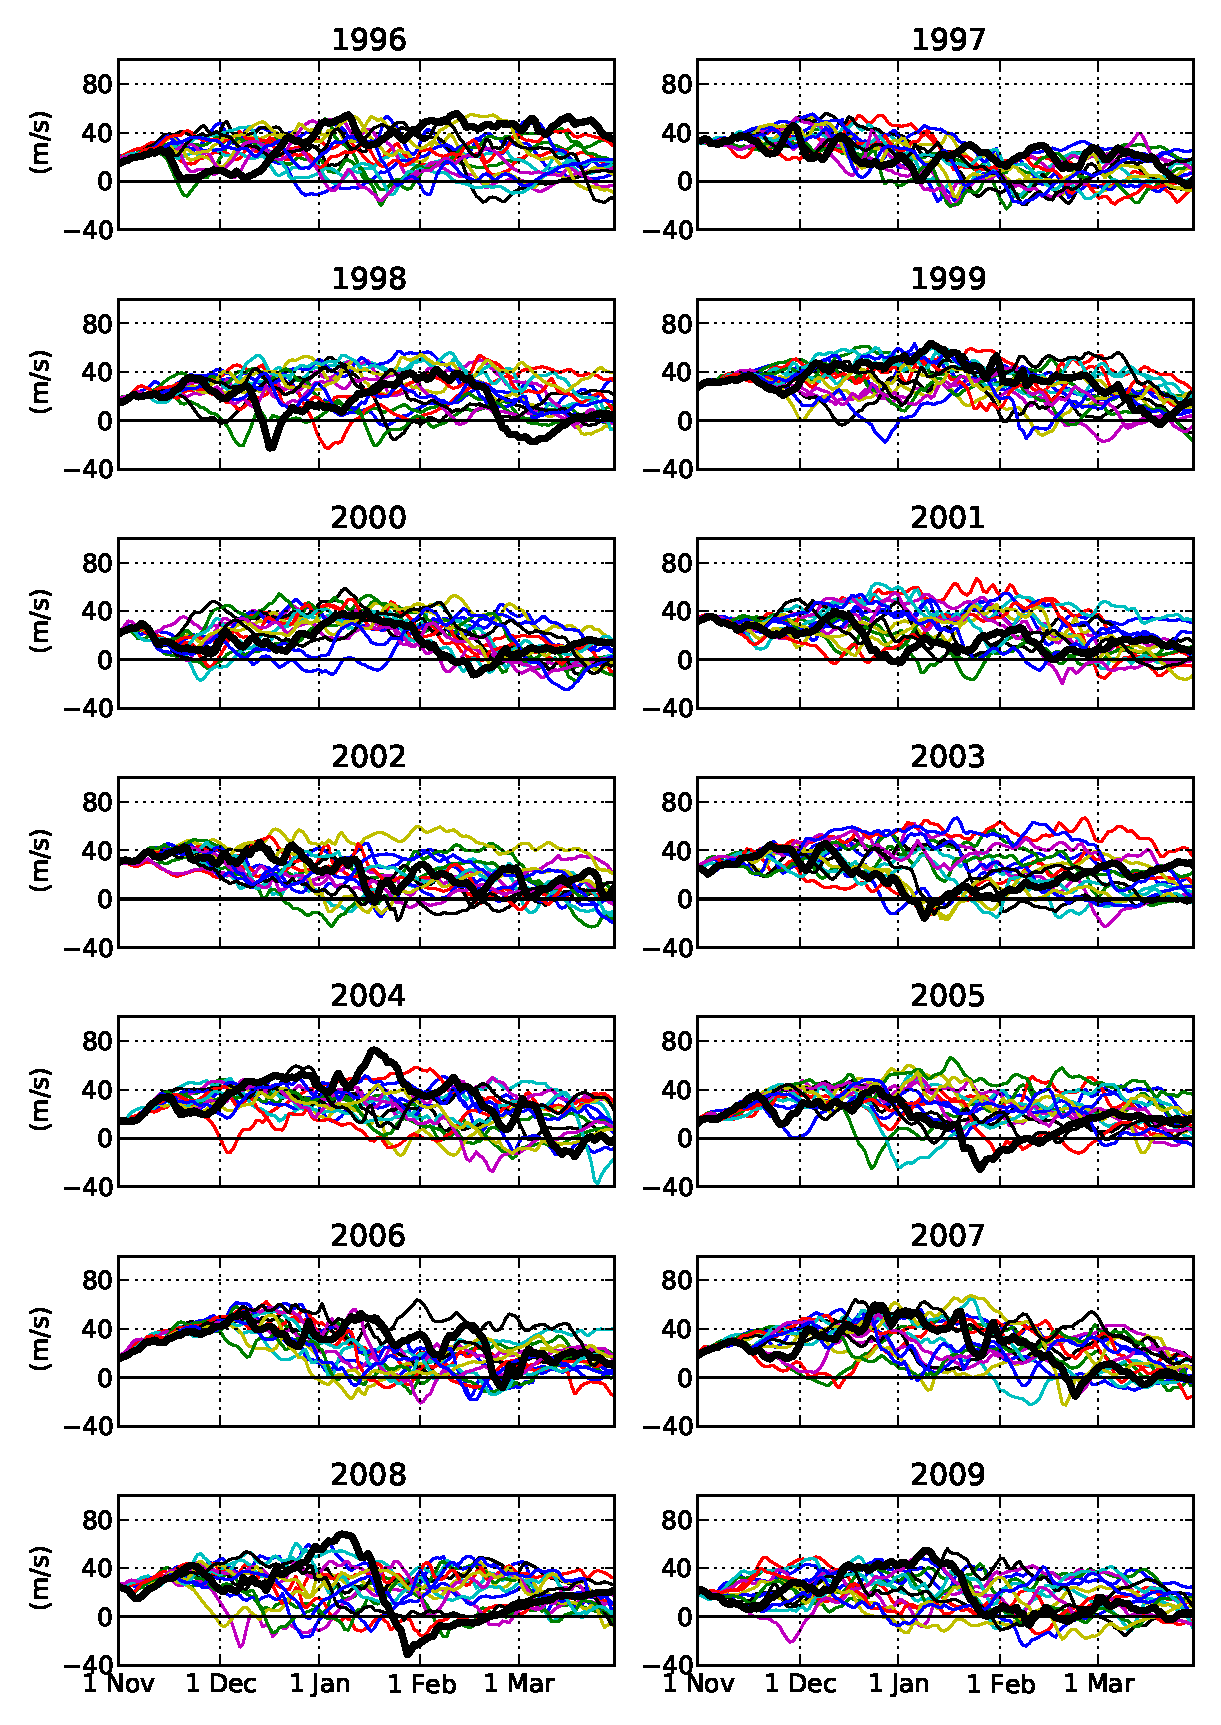
\includegraphics[width=\textwidth]{figures/chapter-seasonal/zm_winds_nh_poststamp.pdf}
   \caption[Timeseries of $\overline{u}$ at 60$^{\circ}$N, 10~hPa, for all
   GloSea5 ensemble members.]{Timeseries of zonal-mean zonal wind in the Arctic
     polar vortex ($60^{\circ}$N, 10~hPa) in the ERA-Interim reanalysis (thick
     black lines) and the GloSea5 ensemble hindcasts (thin coloured
     lines). Individual ensemble members are initialised from dates centred on
     November 1st. Years refer to the year of the initialisation date.}
   \label{fig:nh_poststamp}
\end{figure}

\begin{figure}[p] \vspace*{-3cm} \centering
  \noindent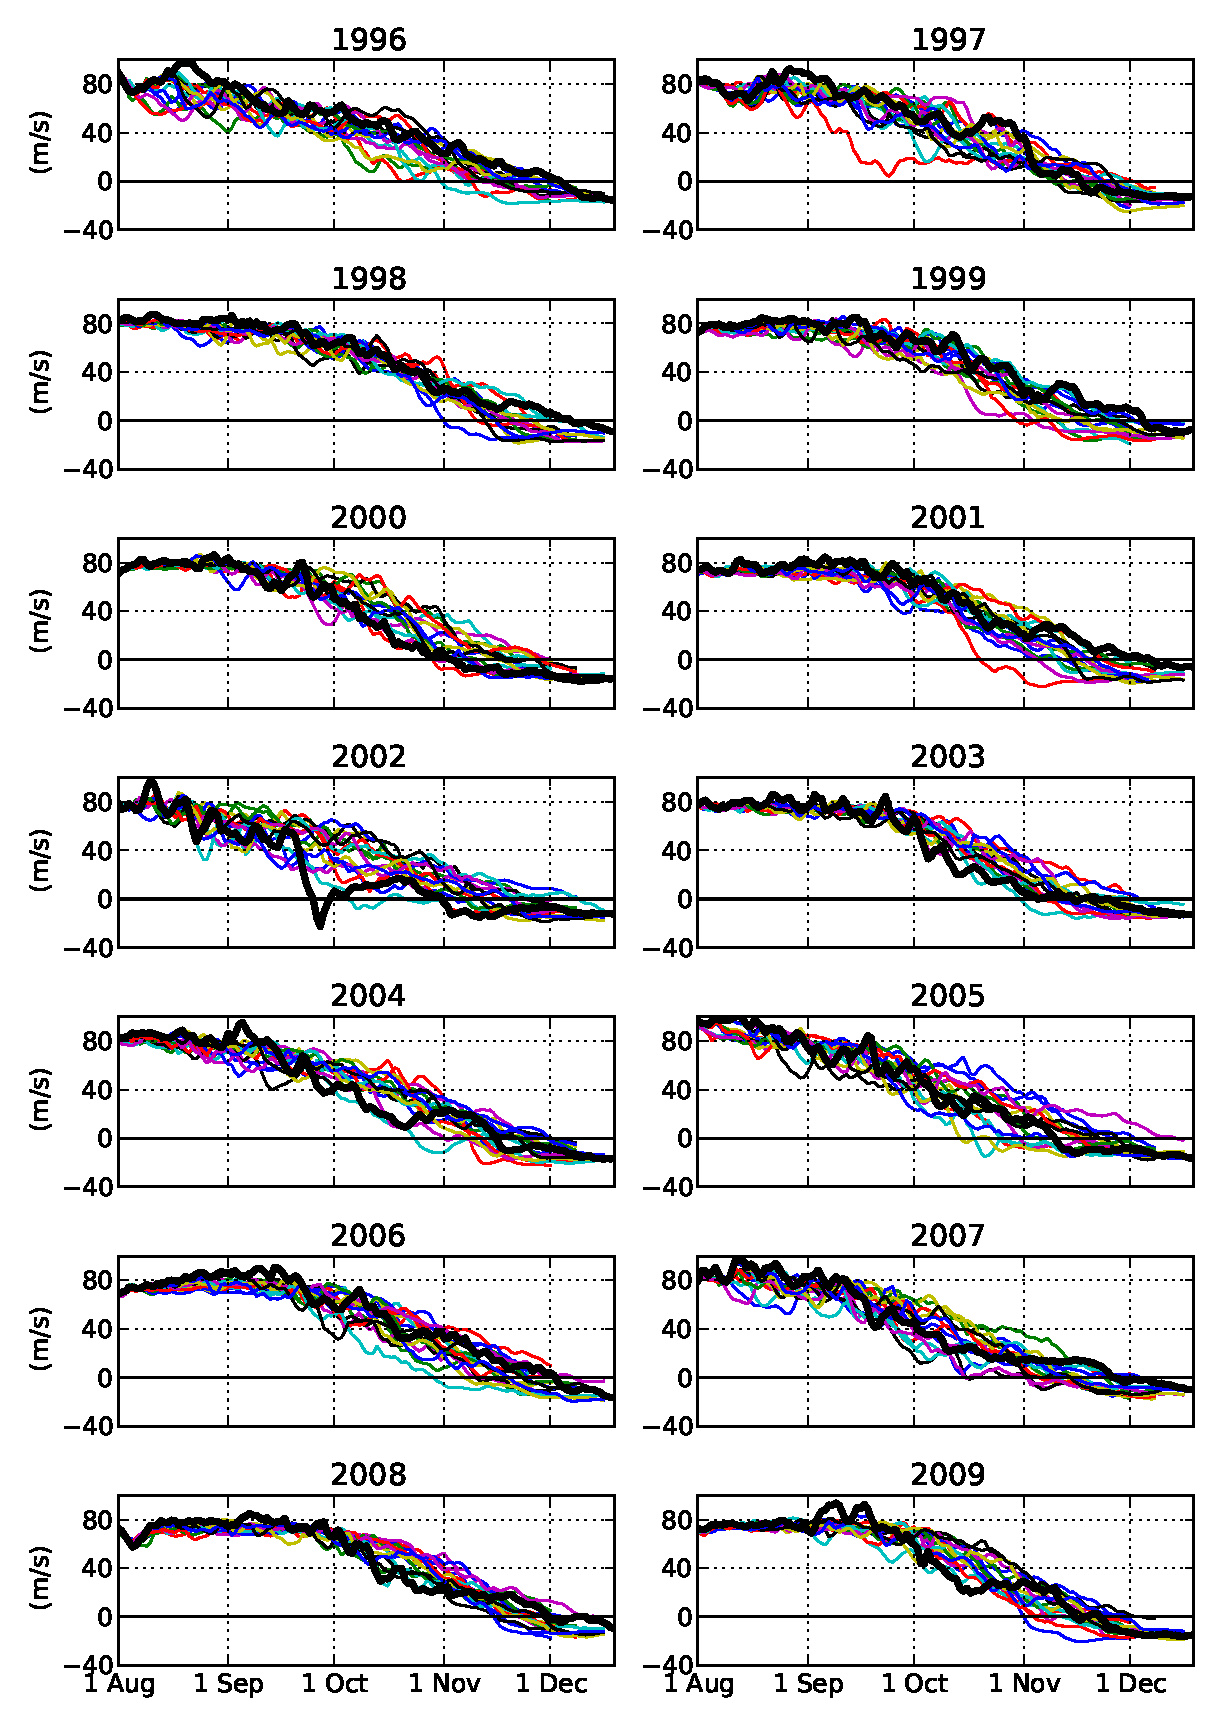
\includegraphics[width=\textwidth]{figures/chapter-seasonal/zm_winds_sh_poststamp.pdf}
  \caption[Timeseries of $\overline{u}$ at 60$^{\circ}$S, 10~hPa, for all
  GloSea5 ensemble members.]{As figure \ref{fig:nh_poststamp} but for the
    zonal-mean zonal wind in the Antarctic polar vortex ($60^{\circ}$S, 10~hPa),
    and ensemble members initialised from dates centred on August 1st.}
  \label{fig:sh_poststamp}
\end{figure}

In order to illustrate these hindcast simulations, timeseries of zonal-mean
zonal wind ($\overline{u}$) at 10~hPa are shown for $60^{\circ}$N from
November--March (Figure \ref{fig:nh_poststamp}) and $60^{\circ}$S from
August--December (Figure \ref{fig:sh_poststamp}). ERA-Interim values are also
shown in both cases (black lines). These are the approximate positions of the
centre of the mean position of the stratospheric polar vortex in the
mid-stratosphere, and therefore indicate the strength of the stratospheric polar
vortex. In order to make the figures comparable, the shorter 14-year, 15-member
ensemble is shown for the NH. It can immediately be seen that there is a much
greater ensemble spread in the NH, owing to the much greater dynamical
variability of the NH stratospheric polar vortex. In both cases it can also be
seen that the ensemble spread is initially small and increases rapidly after
approximately 15-30 days. This demonstrates the initial constraint to
ERA-Interim and the rapid growth of small differences in initial conditions,
because of the chaotic nature of the atmosphere. The predictive skill of for the
Northern Hemisphere (DJF) is analysed in the next section, and the Southern
Hemisphere (SON) in Section \ref{sec:south-hemisph-result}.


\section{Northern Hemisphere results}
\label{sec:north-hemisph-result}
% NH data
% 8.5 events/decade - 3.5 splits, 5.0 displs 
% min 47% (01/02) max 100% (97/98) (any event in winter)

The climatology of Arctic stratospheric polar vortex winds in the GloSea5
hindcasts is compared to the ERA-Interim reanalysis climatology in Figure
\ref{fig:nh_zmzw_clim}. As in Figure \ref{fig:nh_poststamp}, the strength of the
stratospheric polar vortex is measured by the zonal-mean zonal wind
($\overline{u}$) at 60$^{\circ}$N and 10~hPa. The composite for the GloSea5
hindcasts is formed from all the individual ensemble members over the winters
1992/1993--2011/2012 (a total of 480), while that from ERA-Interim is a
composite of the same 20 winters. It can be seen that the mean, interquartile
range and 95th percentile range of the GloSea5 values agree well with the
ERA-Interim values, although the ERA-Interim values are noisier as would be
expected from a sample size consisting of fewer years.

\begin{figure}[t]
  \noindent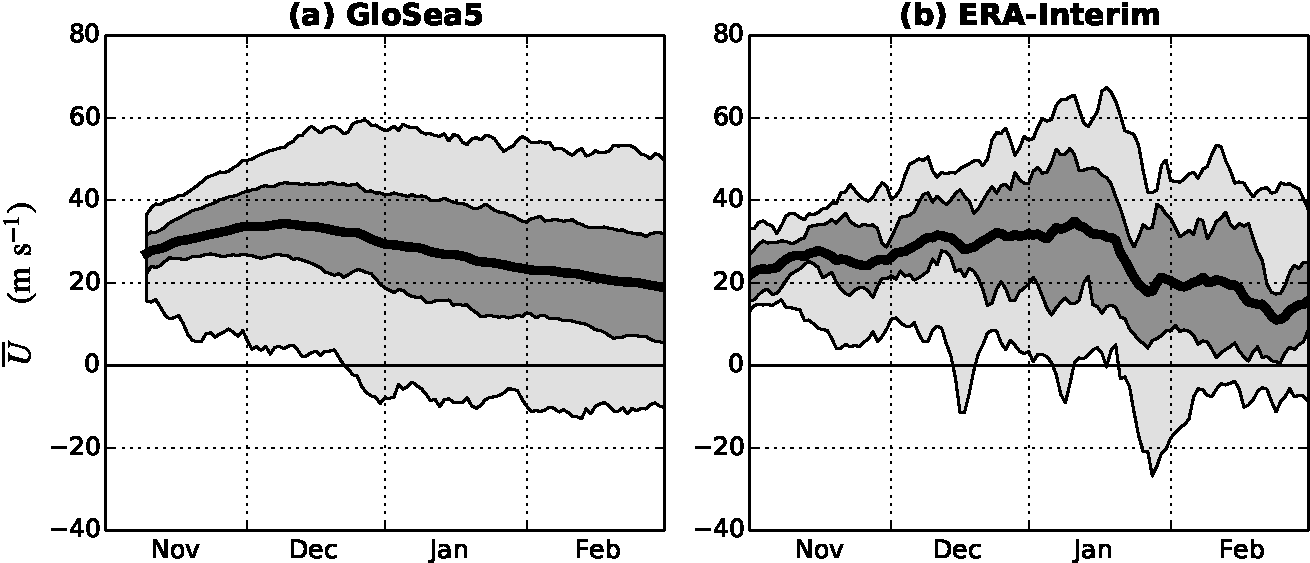
\includegraphics[width=\textwidth,angle=0]{figures/chapter-seasonal/zmzw_climatologies_nh.pdf}\\
  \caption[NH comparison of GloSea5 and ERA-Interim zonal-mean zonal wind
  climatologies.]{Time series of daily 10~hPa zonal-mean zonal wind
    ($\overline{u}$) at 60$^{\circ}$N for all GloSea5 ensemble members (a) and
    ERA-Interim (b) from 1992--2011. The thick black line indicates the mean,
    dark grey shading the interquartile range and light grey the 95th percentile
    range.}\label{fig:nh_zmzw_clim}
\end{figure}

Figure \ref{fig:nh_moments_glosea} shows the joint distribution of the apsect
ratio and centroid latitude moment diagnostics calculated over DJF from the
GloSea5 hindcasts, along with the equivalent values from ERA-Interim. These
diagnostics have been calculated from geopotential height following the method
described in Chapter \ref{cha:moments}. Both aspect ratio and centroid latitude
distributions closely match those of ERA-Interim, and the joint distribution
shows the characteristic triangular shape which is related to the occurrence of
split and displaced vortex events. Together, Figures \ref{fig:nh_zmzw_clim} and
\ref{fig:nh_moments_glosea} demonstrate that GloSea5 accurately simulates the
mean state and variability of the stratospheric polar vortex in the
mid-stratosphere.  

\begin{figure}[t] \centering
  \noindent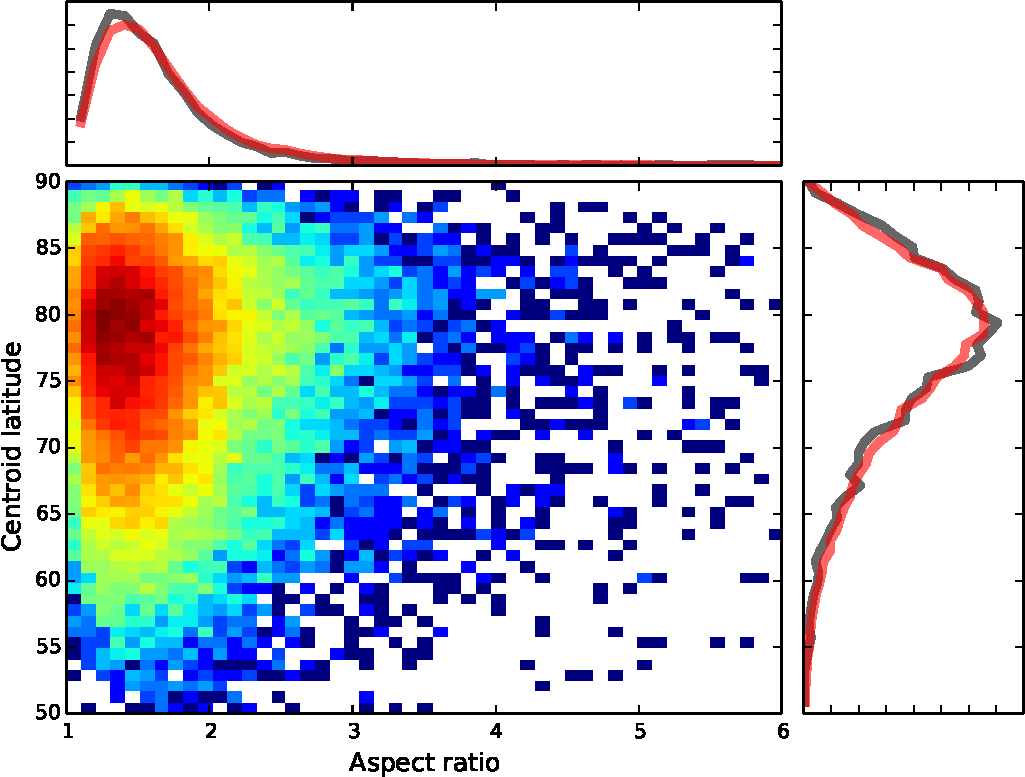
\includegraphics[width=0.7\textwidth,angle=0]{figures/chapter-seasonal/GloSea_moments_histogram.pdf}\\
  \caption[Moment diagnostics for GloSea5.]{Distribution (see Figure
    \ref{fig:cmip5_moments_stats}) of the centroid latitude and aspect ratio
    diagnostics derived from geopotential height for all GloSea5 ensemble
    members (red lines) and ERA-Interim (grey lines) over 1992--2011. The joint
    distribution is plotted with a logarithmic colour scale such that red
    represents the densest regions.}\label{fig:nh_moments_glosea}
\end{figure}

The GloSea5 hindcast predictions of interannual variability of the NH
stratospheric polar vortex winds are shown in Figure
\ref{fig:nh_zmzw_timeseries}. Anomalies are defined from the relevant
climatology of either GloSea5 or ERA-Interim. For GloSea5, this climatology is
calculated from the mean of each day across all ensemble members in all years,
while for ERA-Interim the climatology is the mean of each day, smoothed with a
30-day running mean (in order to account for its increased noise due to the
reduced sample size). Results are shown for DJF averages, corresponding to a 1
month average lead time. The correlation between the GloSea5 ensemble mean and
ERA-Interim is $r=0.24$ which is not statistically significant at the 95\% level
(under the null hypthesis that the two timeseries are
uncorrelated). Significance is calculated using a two-tailed bootstrap test,
whereby the percentile of the observed correlation is calculated from the
distribution of correlations of a large number ($\sim 10~000$) of pairs of time
series formed by re-sampling with replacement from the original time series. As
elswhere in this thesis, these significance tests are used because they make
fewer assumptions about the underlying structure of the data than parametric
tests \citep{Wilks}.

\begin{figure}[t]
  \noindent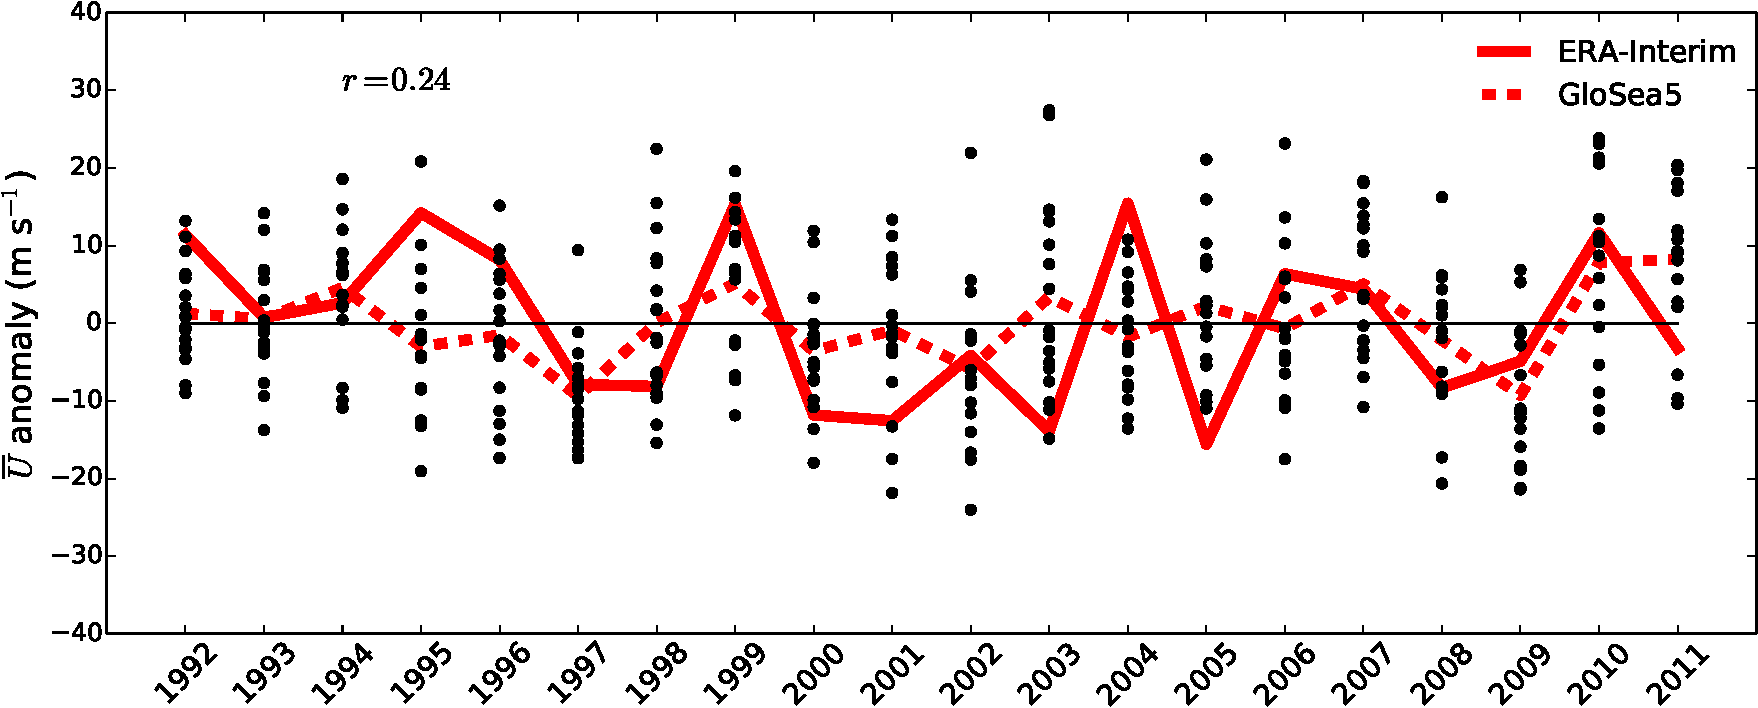
\includegraphics[width=\textwidth,angle=0]{figures/chapter-seasonal/DJF_ZMZW_NH.pdf}\\
  \caption[DJF $\overline{u}$ anomalies for GloSea5.]{DJF mean anomalies of
    $\overline{u}$ at $60^{\circ}$N and 10~hPa for the GloSea5 ensemble mean and
    ERA-Interim. Black dots represent individual ensemble members. The
    correlation between the GloSea5 ensemble mean and ERA-Interim is $r=0.24$,
    which is not statistically significant from zero. Years refer to the year of
    the initialisation date.}\label{fig:nh_zmzw_timeseries}
\end{figure}

Although no significant skill is found in the prediction of the seasonal mean
strength of the stratospheric polar vortex, it might nonetheless be the case
that skilful predictions of SSW events can be made. This is assessed using
receiver operating characteristic (ROC) curves, a standard method in forecast
evaluation, particularly of binary events \citep[e.g.,][]{Wilks}. In order to
calculate the ROC curve, the following procedure is followed:
\begin{enumerate}[1.]
\item For each ensemble member in each year, determine whether an SSW occurs
  (winters with one SSW and two SSWs are treated the same). 
\item Select a threshold for the prediction of an SSW (e.g., 60\% of ensemble
  members forecast an SSW). 
\item For the given threshold determine the fraction of years for which a SSW
  was correctly predicted (``hit rate'') and the fraction for which a SSW was
  predicted but none occurred (``false alarm rate''). 
\item Repeat the steps 2-3 for a range of thresholds from 0-100\%.
\end{enumerate}
In a skilful system the ROC curve should indicate a higher hit rate than false
alarm rate, bending towards the upper left corner of the graph, while a random
forecast will pass along the 1-1 line. 

\begin{figure}[t] \centering
  \noindent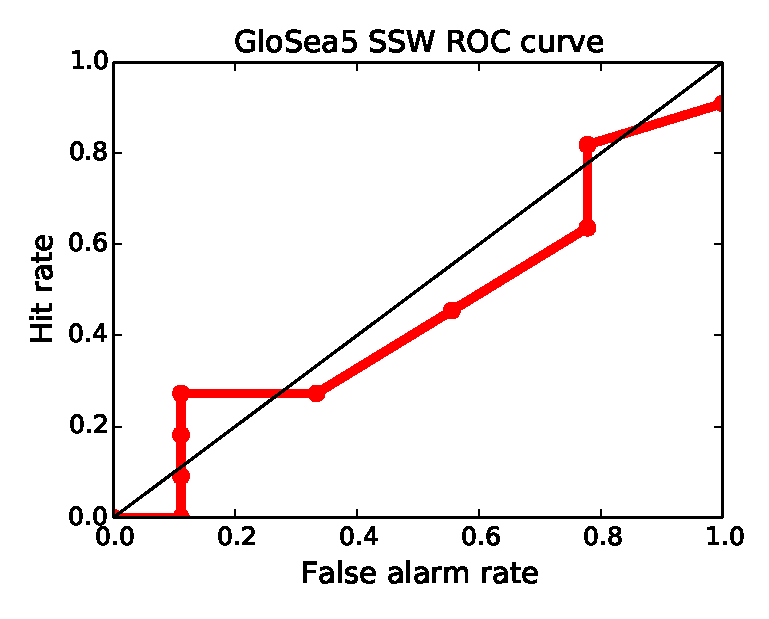
\includegraphics[width=0.5\textwidth,angle=0]{figures/chapter-seasonal/SSW_ROC.pdf}\\
  \caption[ROC curve for the prediction of SSWs.]{Receiver operating
    characteristic (ROC) curve for the prediction of SSW events during DJF for
    1992--2011. SSWs are defined as a reversal to easterly $\overline{u}$ at
    60$^{\circ}$N 10~hPa, and must be separated by at least 30
    days.}\label{fig:ssw_roc}
\end{figure}

Figure \ref{fig:ssw_roc} shows the ROC curve for SSWs during DJF, determined by
the traditional reversal of $\overline{u}$ at 60$^\circ$N 10~hPa, with the
additional criterion that events must be separated by at least 30 days. It can
be seen that the calculated ROC curve lies close to the 1-1 line indicating
little skill in these predictions. This is despite quite large variations in the
fraction of ensemble members predicting SSWS; from 47\% (winter 2001--2002) to
100\% (winter 1997--1998).

\begin{figure}[t] \centering
  \noindent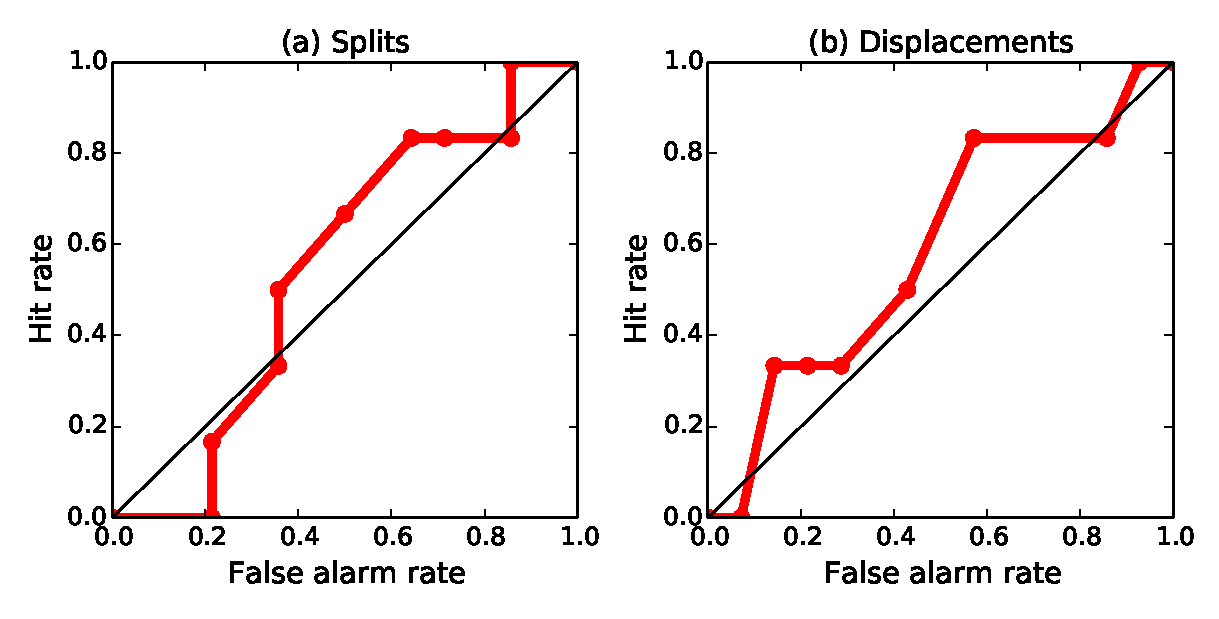
\includegraphics[width=0.8\textwidth,angle=0]{figures/chapter-seasonal/glosea_split_displ_ROC_any.pdf}\\
  \caption[ROC curves for the prediction of split and displaced vortex
  events.]{Receiver operating characteristic (ROC) curves for the prediction of
    split (a) and displaced (b) vortex events in all GloSea5 ensemble members
    over 1992--2011. Split and displaced vortex events are identified from
    geopotential height-derived moment diagnostics using the method described in
    Chapter \ref{cha:moments}.}\label{fig:split_displ_roc}
\end{figure}

A similar analysis for the prediction of split and displaced vortex events is
shown in Figure \ref{fig:split_displ_roc}. These events have been calculated
from the geopotential height-derived moment diagnostics, using the same
procedure as decribed in Chapter \ref{cha:moments}. Again, little skill can be
seen in the predictions of these events, with both ROC curves lying close to the
1-1 line. It should be noted that GloSea5 predicts a high frequency of split and
displaced vortex events (8.5 events/decade; 3.5 split, 5.0 displaced), compared
to the observed value of 7 events/decade. This is perhaps not surprising given
the HadGEM3 model used in GloSea5 is of the same family as HadGEM2-CC, which was
found to have the highest frequency of events in Chapter \ref{cha:models}.

\begin{figure}[t] \centering
  \noindent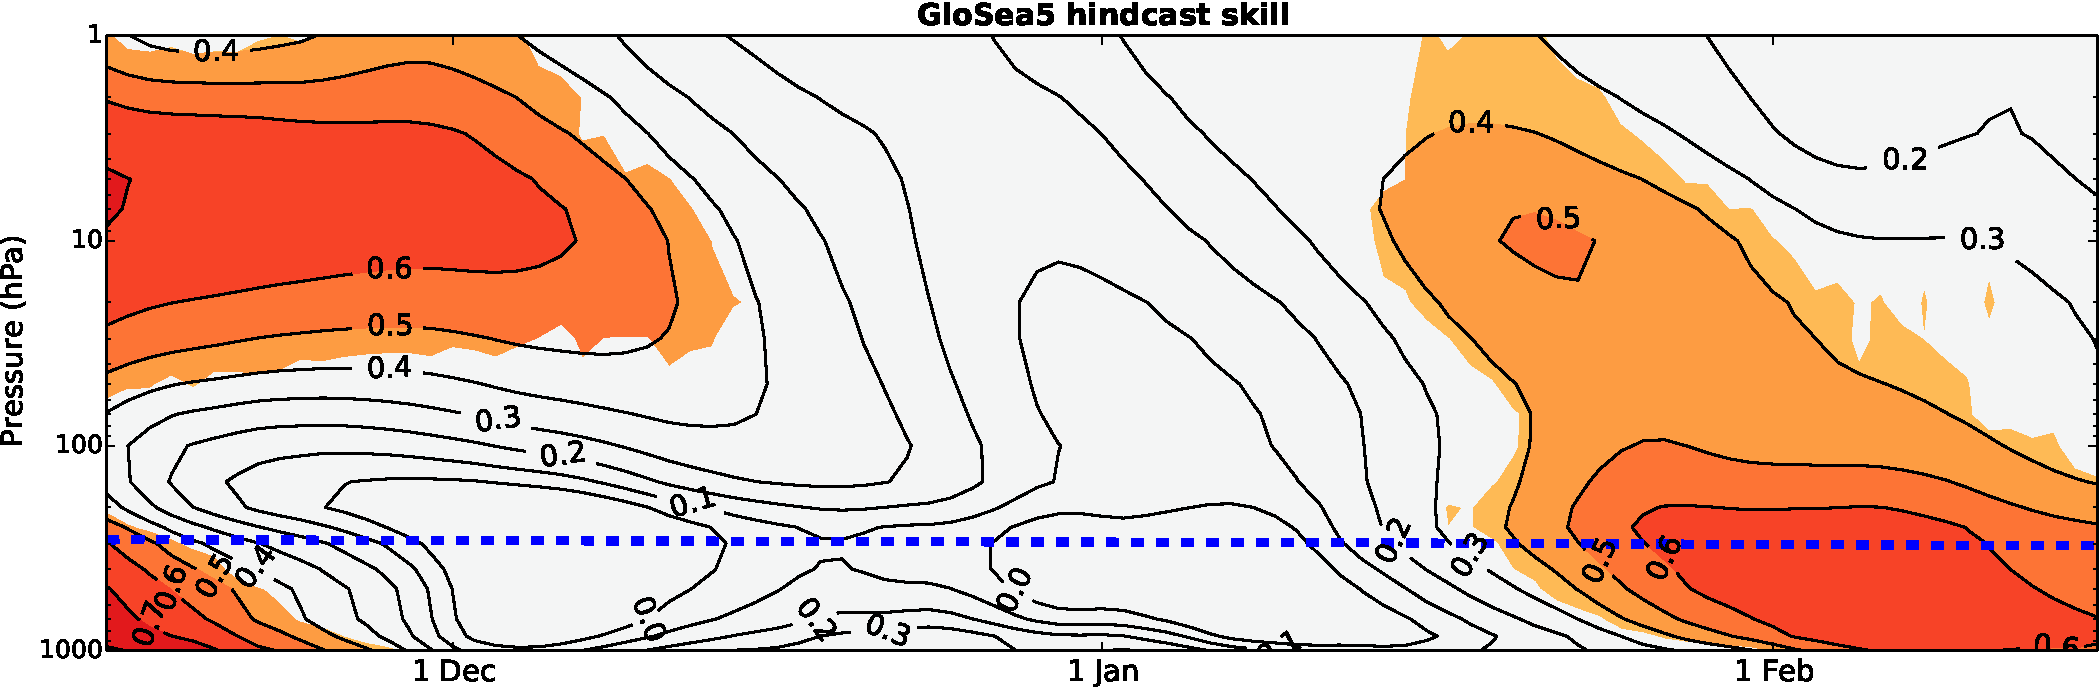
\includegraphics[width=\textwidth,angle=0]{figures/chapter-seasonal/NH_lag_height_corr.pdf}\\
  \caption[Lag-height correlation of NH polar cap geopotential
  height.]{Correlation of GloSea5 ensemble mean polar cap (60-90$^{\circ}$N)
    geopotential height anomalies ($Z'$) with ERA-Interim values from
    1996--2009, as a function of time and height. All values are smoothed with a
    30-day running mean before correlations are calculated. The contour interval
    is 0.1 and all colored regions are greater than zero at the 95\% confidence
    interval, using a bootstrap test at each time at height. The blue dashed
    line indicates the approximate polar cap mean tropopause level
    \citep{Wilcox2012}.}\label{fig:nh_pc_gph_corr}
\end{figure}

\bigskip The evolution of NH hindcast skill as a function of lag and height is
evaluated in Figure \ref{fig:nh_pc_gph_corr}. This shows the correlation of
ERA-Interm and GloSea5 ensemble mean polar cap (60-90$^\circ$N) average
geopotential height anomalies ($Z'$; which is highly correlated with the NAM
\citep{Kushner2010}). Values of $Z'$ are smoothed with a 30-day running mean
before correlations are calculated, and plotted such that values for the 15th
December represent the correlation of the ERA-Interim and GloSea5 ensemble mean
December mean values (without this smoothing, a noisier but similar pattern of
correlations is seen). Geopotential height data on several levels in the
stratosphere is only available in the shorter 14-year, 15-member ensemble, and
so the analysis in this figure is limited to these data. Between 1st-9th
November the ensemble mean is taken as the average of the 10 initialised
ensemble members, and the average of all 15 ensemble members is used after this
date.

In mid-November, significant correlations are seen in Figure
\ref{fig:nh_pc_gph_corr} in both the stratosphere and troposphere, as would be
expected from the initialisation of the hindcasts from ERA-Interim data (skill
is seen to rapidly decay in the tropopause region, however). This skill persists
for longer in the stratosphere than the troposphere, owing to the longer
timescales of stratospheric variability \citep[e.g.,][]{Simpson2011}, however,
by mid-December no significant correlations are seen in the stratosphere or
troposphere. 

Significant correlations return in the troposphere in late Janurary/February,
and to a lesser extent in the stratosphere. This result is similar to that for
the NAO prediction in the same system, which has a greater skill in February
than January (Adam Scaife, Met Office Hadley Centre, personal communication,
2013). A possible explanation for this behaviour is due to the influence of
ENSO, which has been determined to have the greatest effect on the NH
extratropics during late Janurary and February \citep{Bell2009}. If indeed the
influence of ENSO is important, it is not clear whether this arises from a
tropospheric or stratospheric pathway, although the fact that tropospheric skill
is greater than stratospheric may suggest the tropospheric pathway is more
important.

Detailed analysis of the mechanisms behind the NH surface skill is beyond the
scope of this chapter which investigates the role of the stratosphere. Because
skill in the prediction of the NH stratosphere has been demonstrated to be low,
attention is now turned to the SH. However, the implications of these results
are discussed further in Section \ref{sec:seas-discussion}. 


\section{Southern Hemisphere results}
\label{sec:south-hemisph-result}

\subsection{Stratospheric polar vortex}


The climatology of Antarctic stratospheric polar vortex winds in the GloSea5
hindcasts is compared to the ERA-Interim reanalysis climatology in Figure
\ref{fig:sh_zmzw_clim}. The strength of the stratospheric polar vortex is
measured by the zonal-mean zonal wind ($\overline{u}$) at 60$^{\circ}$S and
10~hPa, which is approximately the center of the mean position of the vortex in
the mid-stratosphere. The composite for the GloSea5 hindcasts is formed from all
the individual ensemble members over 1996--2009 (a total of 210), while that
from ERA-Interim is a composite of all years from 1979--2010 (a total of 32
years). It can be seen that the mean of the GloSea5 hindcasts agrees very
closely with ERA-Interim throughout the spring, with only a slight bias towards
weaker winds in August and September. The interquartile and 95th percentile
ranges of GloSea5 and ERA-Interim also agree well, although the ERA-Interim
values are noisier as would be expected from a sample size consisting of fewer
years.

\begin{figure}[t]
  \noindent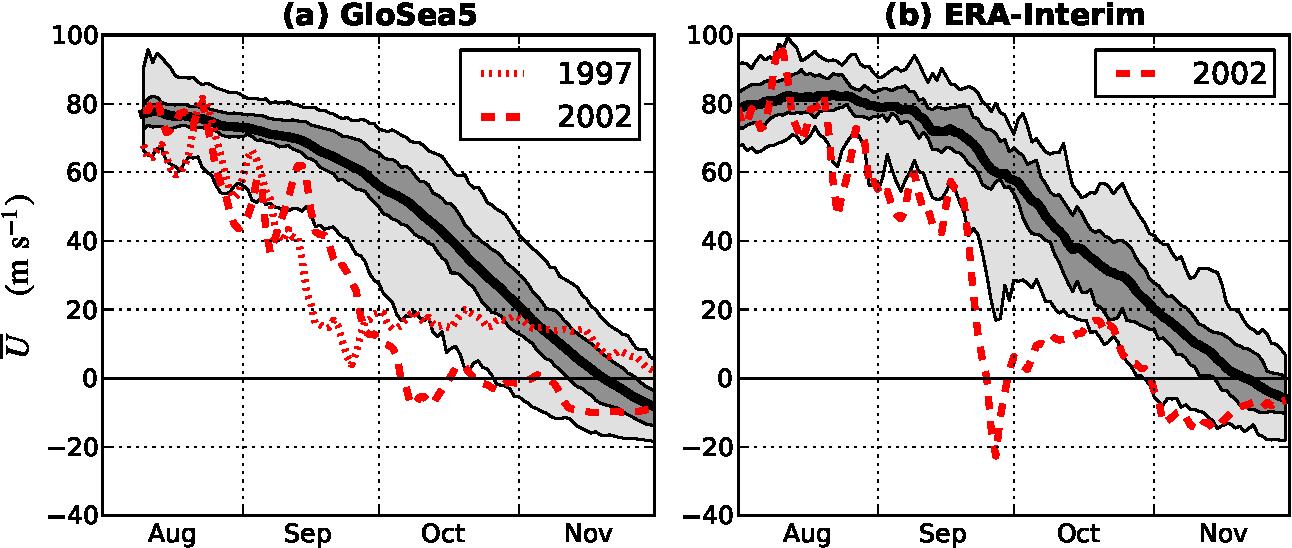
\includegraphics[width=\textwidth,angle=0]{figures/chapter-seasonal/zmzw_climatologies_crop.pdf}\\
  \caption[Comparison of GloSea5 and ERA-Interim zonal-mean zonal wind
  climatologies.]{Time series of daily 10~hPa zonal-mean zonal wind
    ($\overline{u}$) at 60$^{\circ}$S for all GloSea5 ensemble members from
    1996--2009 (a) and ERA-Interim from 1979--2010 (b). The thick black line
    indicates the mean, dark gray shading the interquartile range and light gray
    the 95th percentile range. Individual time series of the ensemble member of
    GloSea5 for 2002 which simulated an SSW, and 1997 which simulated a
    near-SSW, and the year with an observed SSW (2002) are shown in
    red.}\label{fig:sh_zmzw_clim}
\end{figure}

The GloSea5 hindcast predictions of interannual variability of the Antarctic
stratospheric polar vortex winds are shown in Figure
\ref{fig:zmzw_ozone}(a). Anomalies are defined from the relevant climatology of
either GloSea5 or ERA-Interim. For GloSea5, this climatology is calculated from
the mean of each day across all ensemble members in all years, while for
ERA-Interim the climatology is the mean of each day, smoothed with a 30-day
running mean (in order to account for its increased noise due to the reduced
sample size). Results are shown for September--November (SON) averages,
corresponding to a 1 month average lead time. The correlation between the
GloSea5 ensemble mean and ERA-Interim is 0.73, which is statistically
significant from zero at the 99\% confidence level, and has a 95\% confidence
interval of (0.37, 0.90). This correlation does not depend strongly on particular
years; the correlation remains significant at the 95\% level ($r=0.57$) if the
year 2002 (which has the greatest anomaly) is excluded. Significance is
calculated using a two-tailed bootstrap test, whereby the percentile of the
observed correlation is calculated from the distribution of correlations of a
large number ($\sim 10,000$) of pairs of time series formed by re-sampling with
replacement from the original time series. These significance tests make fewer
assumptions about the underlying structure of the data than parametric tests
\citep{Wilks}, and are used throughout this study.

\begin{figure}[t]
  \noindent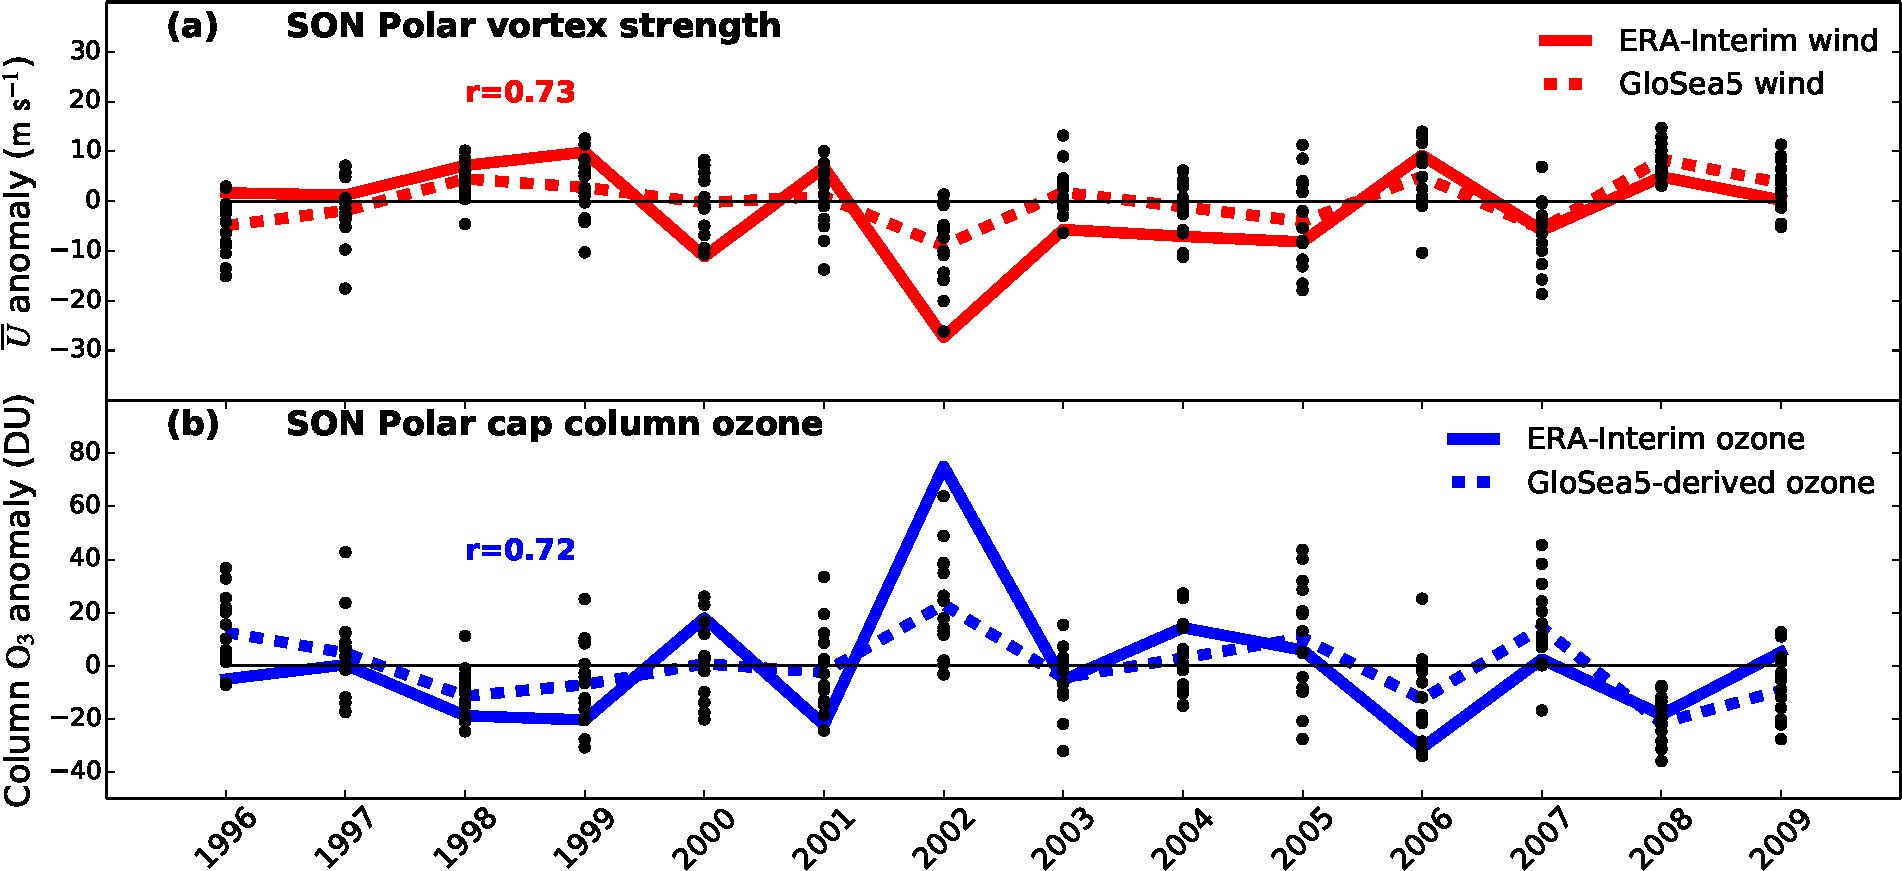
\includegraphics[width=\textwidth,angle=0]{figures/chapter-seasonal/zmzw_ozone_crop.pdf}\\
  \caption[GloSea5 forecast skill for the stratospheric polar vortex strength
  and column ozone.]{(a) SON mean anomalies at 10~hPa and 60$^{\circ}$S in
    ERA-Interim and the GloSea5 hindcast ensemble mean. (b) SON mean polar cap
    averaged (60--90$^{\circ}$S) total column ozone anomalies from ERA-Interim
    and those derived from the GloSea5 anomalies as described in the
    text. Individual ensemble members are shown as black dots. Hindcasts are
    initialized near 1st August.}\label{fig:zmzw_ozone}
\end{figure}

The skill shown in Figure \ref{fig:zmzw_ozone}(a) cannot be accounted for by
persistence of initial anomalies. In fact, there is a negative correlation
between $\overline{u}$ on 9th August, when the last ensemble member is
initialised, and the SON mean ($r=-0.54$). Hence, a persistence forecast would
be negatively correlated with observed values. This relationship may be
consistent with ideas of a pre-conditioning of the polar vortex \citep[e.g.,][
Section \ref{sec:strat-sudd-warm}]{McIntyre1983}. The standard deviation of all
GloSea5 ensemble members is $7.5~\mathrm{m~s^{-1}}$ and that of ERA-Interim is
$9.7~\mathrm{m~s^{-1}}$ indicating that the GloSea5 ensemble spread may be too
small. However, there are large uncertainties in these values due to the short
hindcast period and the large 2002 anomaly.

Following \citet{Charlton2007}, SSWs are defined as a temporary reversal of
$\overline{u}$ at 60$^{\circ}$S and 10~hPa, occurring before the final
transition to summer easterlies (final warming). Under this definition, one SSW
event was simulated in the GloSea5 hindcasts, in 2002. A similar magnitude event
(in terms of departure from climatology) occurred in a 1997 ensemble member,
although $\overline{u}$ did not quite become easterly. Time series of
stratospheric polar vortex winds for these two events are shown in Figure
\ref{fig:sh_zmzw_clim}(a) along with the observed 2002 SSW in Figure
\ref{fig:sh_zmzw_clim}(b). It can also be seen in Figure
\ref{fig:sh_zmzw_clim}(a) that 2002 has the most anomalous stratospheric polar
vortex in the GloSea5 hindcasts, with 14 of 15 ensemble members simulating
negative anomalies, and the most negative ensemble mean. It is therefore
possible that an increased likelihood the 2002 event was to some degree
detectable about two months in advance, although it has not been determined
whether this predictability comes from a preconditioning of the vortex, as
suggested by \citet{Scaife2005c}, or the result of external forcing.

Both the SSW events simulated by GloSea5 were vortex displacement events, in
contrast to the vortex splitting event which occurred in 2002
\citep{Charlton2005a}. This is demonstrated in Figure \ref{fig:sh_ssws}, which
shows geopotential height in the mid-stratosphere at the date of minimum
$\overline{u}$ at 60$^{\circ}$S and 10~hPa, for the two simulated events in
GloSea5 and the observed event in ERA-Interim. A detailed quantitative anaysis
using moment diagnostics was not found necessary in this case because a
qualitative inspection is possible with only two events.

\begin{figure}[t]
  \noindent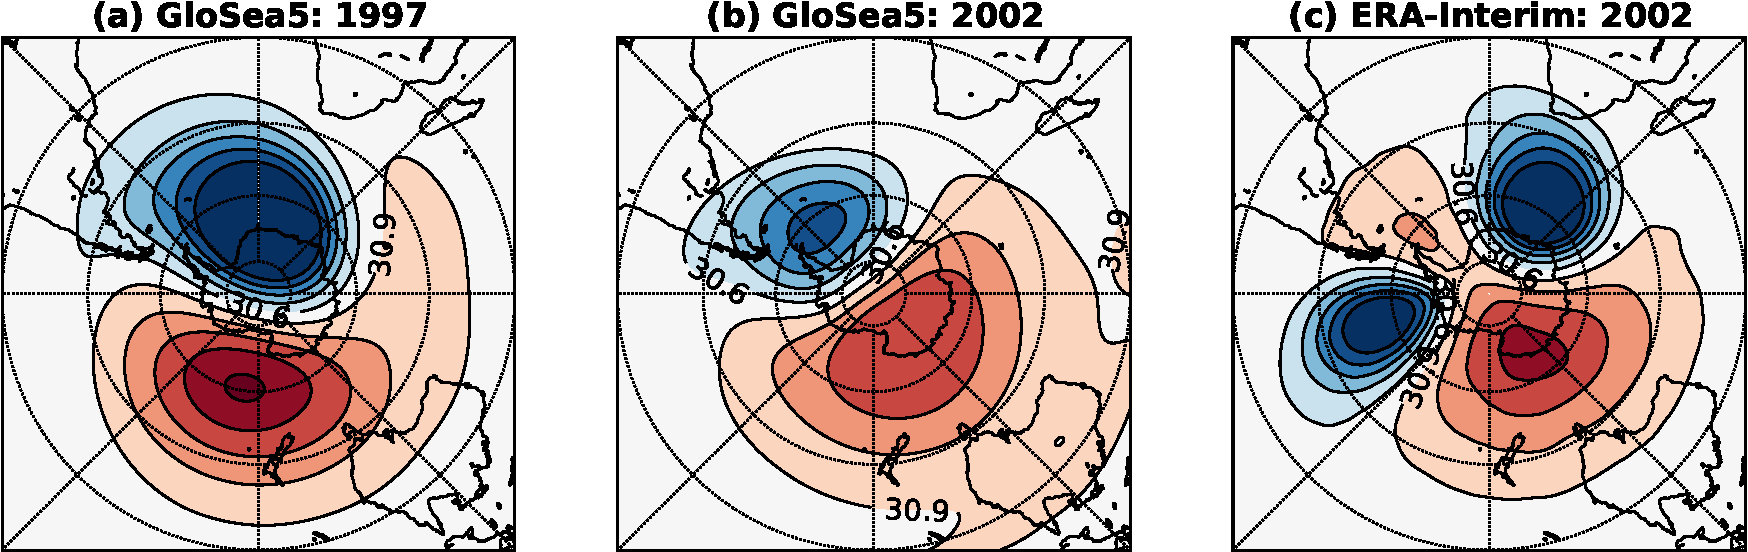
\includegraphics[width=\textwidth,angle=0]{figures/chapter-seasonal/ssws_crop.pdf}\\
  \caption[Comparison of GloSea5 and observed SSWs.]{Geopotential height at
    10~hPa on the date at which $\overline{u}$ at 60$^{\circ}$S and 10~hPa is at
    its minimum value, for the two GloSea5 ensemble members which simulate a SSW
    (a,b), and for ERA-Interim at the central date of the 2002 SSW (c). Units
    are km and the contour interval is 0.3~km.}\label{fig:sh_ssws}
\end{figure}

The timing of the final warming of the stratospheric polar vortex also has a
significant effect on stratospheric temperature and ozone concentrations
\citep{Yamazaki1987}, as well as on the coupling of the stratosphere to the
troposphere \citep{Black2007}. The predictability of these events was
investigated in GloSea5, but not found to be highly significant. This is
probably because the mean timing of the final warming is towards the end of the
four month hindcast simulation (around 20th November at 10~hPa), and the final
warming does not occur before the end of the hindcast for some ensemble members,
thereby introducing a bias in the mean.

\subsection{Ozone depletion}
\label{sec:ozone-depletion}

GloSea5 does not include interactive ozone chemistry, so in order to make ozone
forecasts concentrations must be inferred from other meteorological
variables. Total ozone quantities over the Antarctic polar cap have been found
to be highly correlated with vertical EP flux poleward of 40$^{\circ}$S
\citep{Weber2011, Salby2012}. EP flux diagnostics are not routinely produced
directly by operational seasonal forecast systems and requires high frequency
output at high spatial resolution to calculate. However, vertical EP flux
dominates variability of the stratospheric polar vortex, so it may be possible
to use the strength of the vortex to infer ozone quantities.

SON mean total column ozone quantities area-weighted averaged over the polar cap
(60--90$^{\circ}$S) are shown in Figure \ref{fig:zmzw_scatter}(a) for
ERA-Interim and the Total Ozone Mapping Spectrometer (TOMS) satellite instrument
\citep{Kroon2008}. ERA-Interim data are highly correlated with TOMS, verifying
the accuracy of ERA-Interim against direct satellite measurements (TOMS values
are slightly higher than ERA-Interim; this is probably because TOMS cannot make
observations during the polar night). The long-term trend in polar cap total
column ozone is calculated by fitting a second-order polynomial to the
data. This long-term trend is due to changes in concentrations of CFCs and other
ozone-depleting substances, and largely unrelated to dynamical variability. On
the other hand, shorter-term interannual changes are strongly related to
dynamical variability. In Figure \ref{fig:zmzw_scatter}(b) anomalies of polar
cap total column ozone from the long-term trend are plotted against anomalies of
the SON mean $\overline{u}$ at 60$^{\circ}$S and 10~hPa. It can be seen that
these two quantities are highly correlated ($r=-0.92$), meaning polar vortex
variability explains approximately 85\% of the variance of polar cap total
column ozone anomalies.

\begin{figure}[t]
  \noindent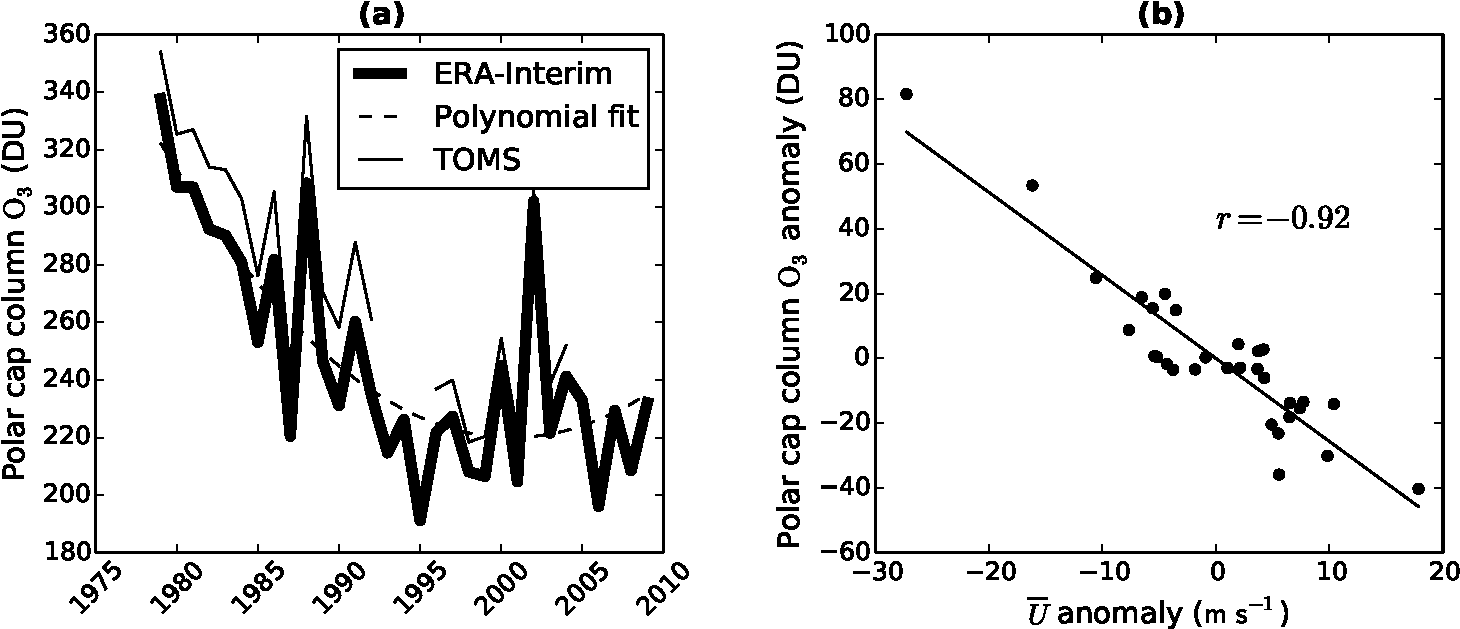
\includegraphics[width=\textwidth,angle=0]{figures/chapter-seasonal/zmzw_ozone_scatter_crop.pdf}\\
  \caption[Relation between stratospheric polar vortex strenth and column
  ozone.]{(a) Time series of SON mean polar cap averaged (60-90$^{\circ}$S)
    total column ozone in ERA-Interim and the TOMS satellite instrument. The
    ERA-Interim data are fitted with a 2nd-order polynomial. (b) Anomalies of
    ERA-Interim column ozone from the polynomial fit plotted against SON mean
    anomalies at 10~hPa and 60$^{\circ}$S for each year from
    1979--2009.} \label{fig:zmzw_scatter}
\end{figure}

This strong correlation makes it possible to use GloSea5 forecasts of polar
vortex winds to produce inferred predictions of polar cap total column ozone
quantities. This is carried out by a leave-one-out cross-validation procedure
\citep{Wilks}; the linear regression of ERA-Interim ozone and $\overline{u}$
anomalies for all years 1979--2009 except the hindcast year is used to produce
the hindcast for each ensemble member. Thus no information from the hindcast
year enters the hindcast itself. Figure \ref{fig:zmzw_ozone}(b) shows the
GloSea5 ozone hindcasts along with the assimilated values from ERA-Interim. The
correlation between the GloSea5 ensemble mean and ERA-Interim is 0.73, which is
statistically significant at the 99\% level, and has a 95\% confidence interval
of $(0.38,0.91)$. Errors from the regression in Figure \ref{fig:zmzw_ozone}(b)
for the inferred ozone quantities for each ensemble member are small compared to
the spread between ensemble members, and so are not plotted in this figure.

\subsection{Southern Annular Mode}

The SAM index in both GloSea5 and ERA-Interim is depicted as the difference
between the normalized anomalies of zonally averaged mean sea-level pressure at
40$^{\circ}$S and 65$^{\circ}$S \citep{Gong1999}. These anomalies are calculated
from the respective climatologies of GloSea5 and ERA-Interim. The ERA-Interim
SAM index calculated in this way is also highly correlated with other measures
of the SAM, such as the station-based index of \citet{Marshall2003}. The GloSea5
hindcast skill for the prediction of the seasonal (SON) mean SAM index is shown
in Figure \ref{fig:sam_ts} . The correlation of the GloSea5 ensemble mean and
ERA-Interim is 0.64, which is statistically significant at the 95\% level, and
has a 95\% confidence interval of (0.18,0.92) confirming skillful prediction of
the SAM at 1 month average lead times. This is similar to the value for the
December--February (DJF) NAO correlation skill of 0.62 found by
\citet{Scaife2013} in the same seasonal forecast system. The 1-year lag
autocorrelation of the SON mean SAM is negative ($r=-0.36$), and accounting for
this by sampling pairs of consecutive years in the bootstrap test leads to a
narrower confidence interval than presented above. The variability of the SAM
simulated by GloSea5 is broadly realistic with a standard deviation of all
ensemble members of 0.98 compared to 0.90 in ERA-Interim over the same period.

The SAM is strongly related to surface temperatures over much of the SH
extratropics. Figure \ref{fig:mslp_tsrf_map}(a) shows the correlation of the SON
mean SAM from ERA-Interim over 1996--2009 with SON mean gridded station-based
surface temperature data from the HadCRUT4 data set \citep{Morice2012}. The
HadCRUT4 data set has been chosen to demonstrate the relationship between the
SAM and surface temperature because of the scarcity of temperature observations
in the Southern Hemisphere, meaning reanalysis data is poorly constrained in
many regions. The same relationship between surface temperatures and the SAM is
shown for the GloSea5 ensemble mean in Figure \ref{fig:mslp_tsrf_map}(b). Many
of the observed correlations are reproduced in the hindcasts, such as the
opposite signed correlations over east Antarctica and the Antarctic
Peninsula/Patagonia, as well as between eastern Australia and New Zealand. These
results are in agreement with \citet{Gillett2006} who analysed the temperature
patterns associated with the SAM over the longer observational record of
1957--2005.

\begin{figure}[t]
  \noindent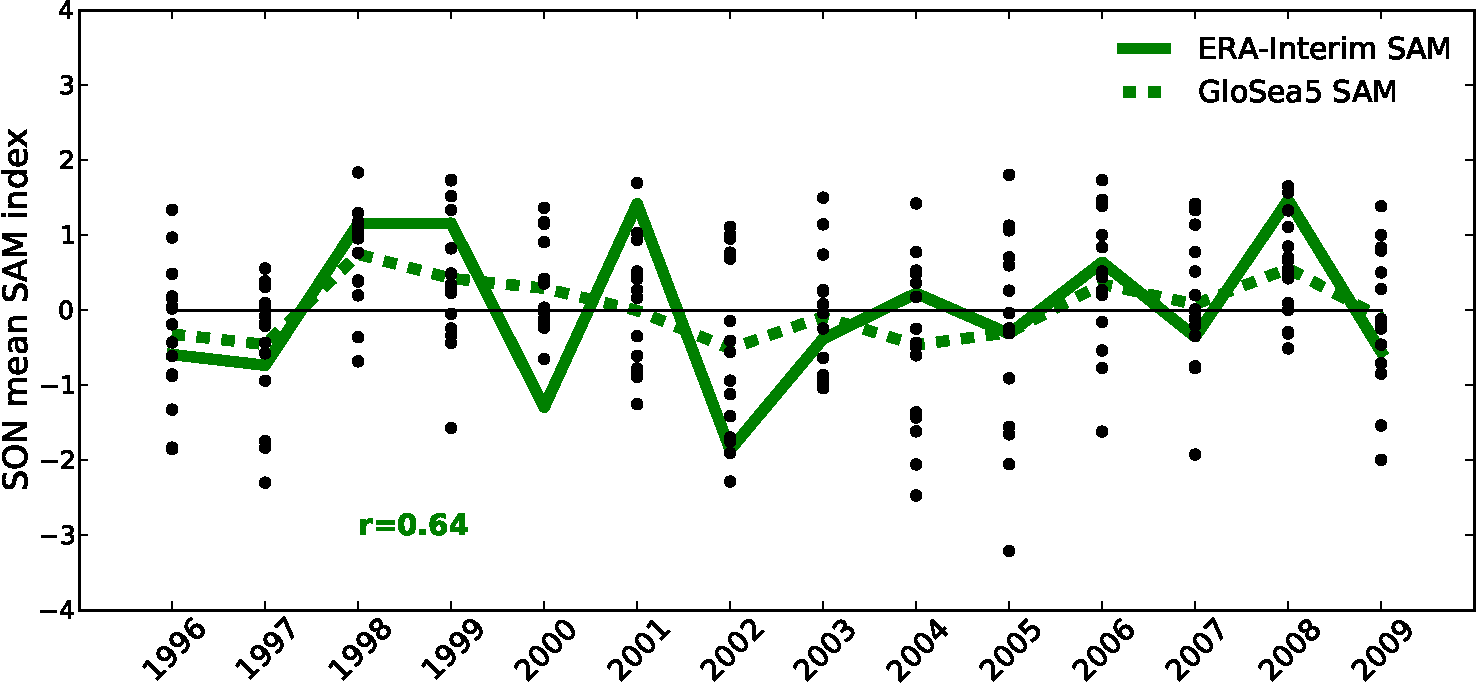
\includegraphics[width=\textwidth,angle=0]{figures/chapter-seasonal/sam_crop.pdf}\\
  \caption[GloSea5 predictions of the SAM.]{SON mean Southern Annular Mode (SAM)
    index in individual GloSea5 hindcast ensemble members (dots), ensemble mean
    (dashed green curve) and ERA-Interim (solid green curve). The SAM is
    calculated from mean sea-level pressure data, and hindcasts initialized near
    1st August. The correlation of the ensemble mean and ERA-Interim values is
    0.64, which is statistically significant at the 95\%
    level.}\label{fig:sam_ts}
\end{figure}

The GloSea5 ensemble mean SON surface temperature correlation with HadCRUT4 is
shown in Figure \ref{fig:mslp_tsrf_map}(c). Also highlighted (black circles) are
the points with the strongest observed correlations with the SAM ($|r| > 0.5$).
Regions of significant positive correlations are found over east Antarctica,
Patagonia, New Zealand, and eastern Australia. These are regions which also have
a strong correlation with the SAM, indicating that the significant surface
temperature skill is related to skill in prediction of the SAM. On the other
hand, there are also some significant negative correlations in subtropical
regions, which may indicate a model bias in the temperature pattern associated
with the SAM in these regions.

\begin{figure}[t]
  \noindent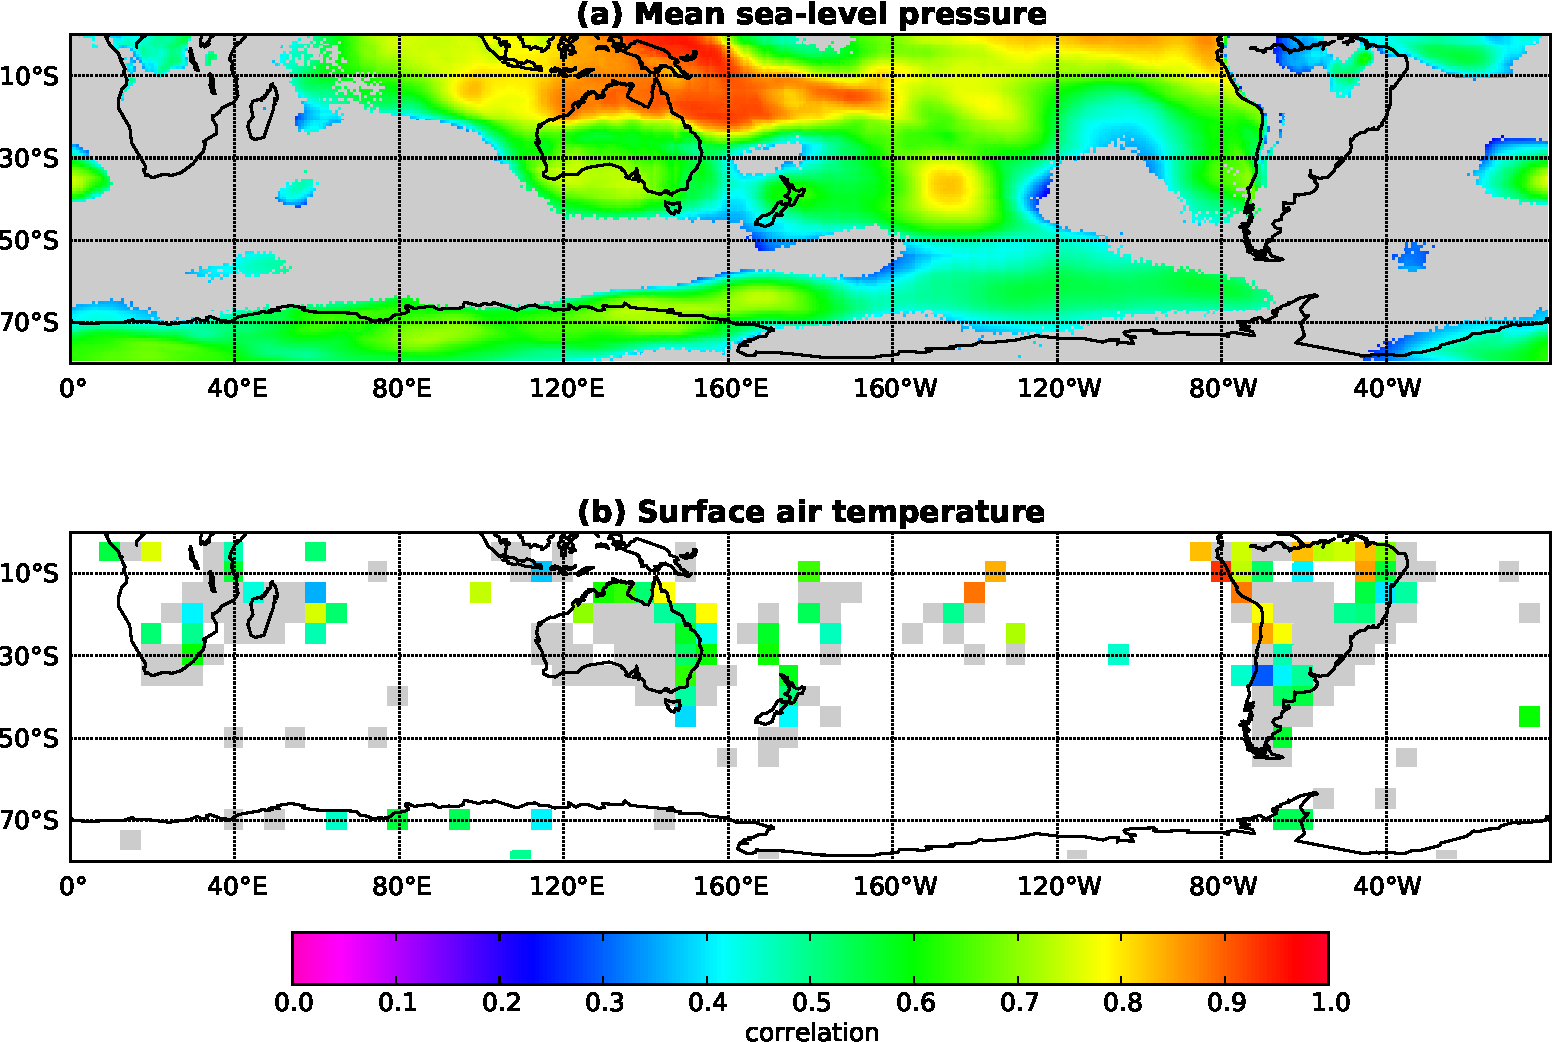
\includegraphics[width=\textwidth,angle=0]{figures/chapter-seasonal/mslp_tsrf_maps_crop.pdf}\\
  \caption[Correlation of GloSea5 forecasts of sea-level pressure and
  temperature.]{(a) Correlation of the ERA-Interim SON mean SAM with SON mean
    HadCRUT4 gridded station-based temperature observations over 1996--2009. (b)
    Correlation of the SON GloSea5 ensemble mean hindcast SAM with the SON
    hindcast ensemble mean near-surface temperature. (c) Correlation of observed
    SON mean HadCRUT4 and hindcast GloSea5 ensemble mean temperature. In (c)
    only correlations which are significant from zero at the 95\% level
    according to a bootstrap test at each gridpoint are shown. Black circles
    represent points which have an observed correlation with the SAM with
    magnitude greater than 0.5.}\label{fig:mslp_tsrf_map}
\end{figure}


\subsection{Stratosphere-troposphere coupling}
\label{sec:seas-strat-trop-coupl}

It is now investigated whether the statistically significant skill in hindcasts
of the stratospheric polar vortex affects that of the surface SAM. Forecast
skill as a function of lead-time and height is studied for polar cap
(60-90$^{\circ}$S) mean geopotential height anomalies ($Z'$)\footnote{Throughout
  the troposphere and stratosphere daily $Z'$ is highly correlated ($r>0.9$)
  with the SAM index calculated from zonal mean geopotential height
  \citep{Baldwin2009}.}. Figure \ref{fig:gph_lag_corr}(a) shows the correlation
of $Z'$ in ERA-Interim with the GloSea5 ensemble mean hindcast values. Values
are smoothed with a 30-day running mean before correlations are calculated, and
plotted such that values for 15th September represent the correlation of the
ERA-Interim and GloSea5 ensemble mean September mean values (without this
smoothing, there are noisier but still significant correlations in a similar
pattern). Between 1st-9th August the ensemble mean is taken as the average of
the 10 initialized ensemble members, and the average of all 15 ensemble members
is used after this date.

\begin{figure}
  \centering
  \noindent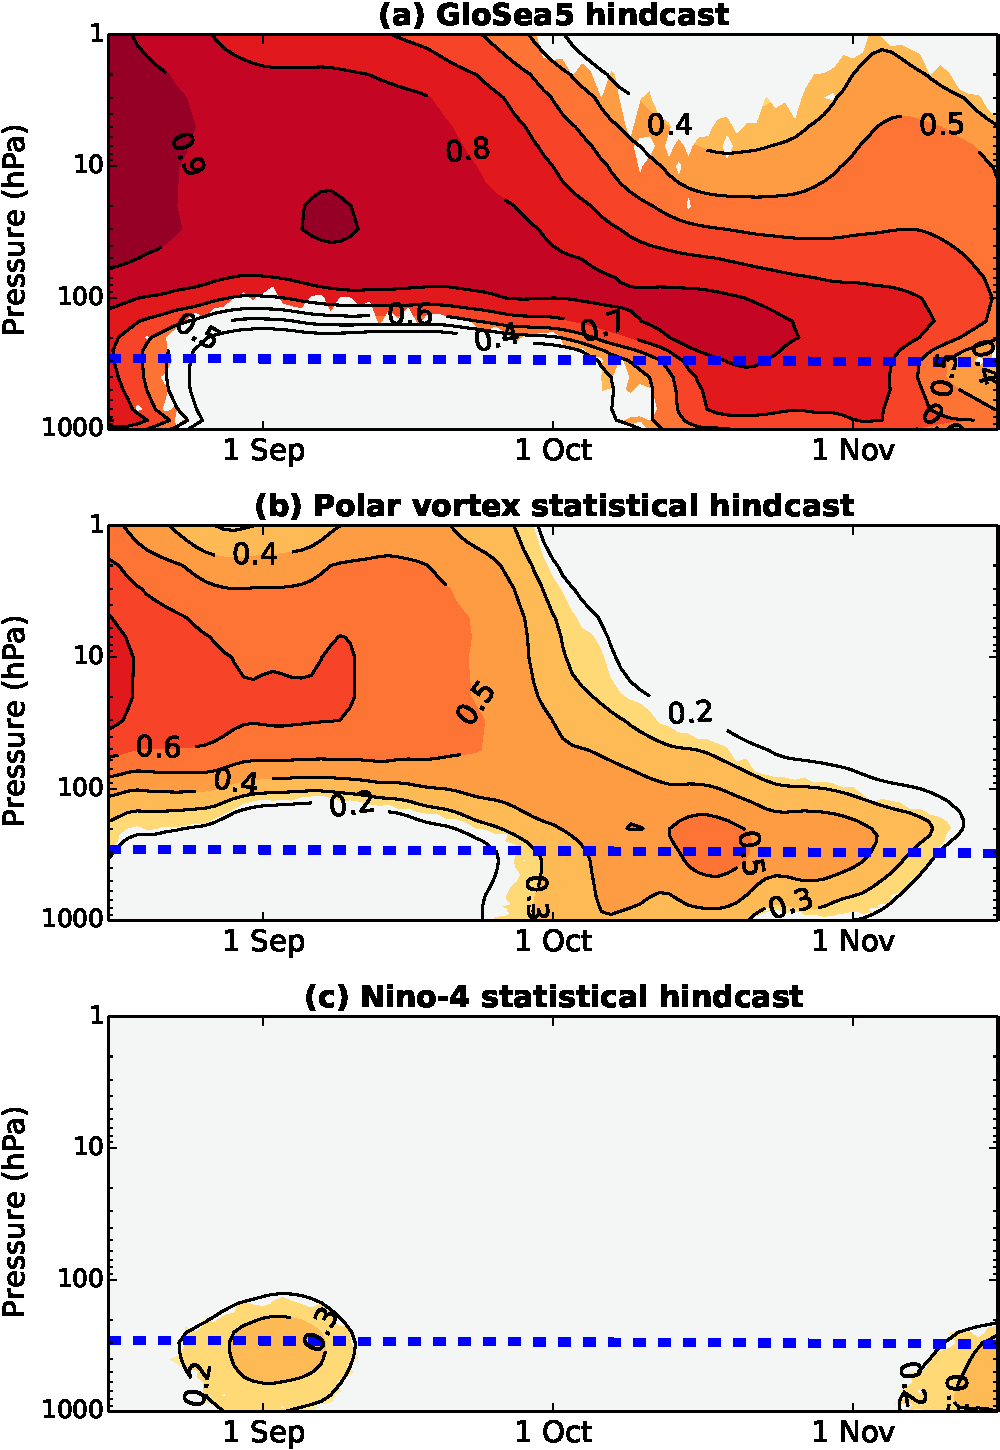
\includegraphics[width=0.7\textwidth,angle=0]{figures/chapter-seasonal/lag_corr_crop_vert.pdf}\\
  \caption[Lag-height correlation of GloSea5 polar cap geopotential height]{(a)
    Correlation of GloSea5 ensemble mean polar cap (60-90$^{\circ}$S)
    geopotential height anomalies ($Z'$) with ERA-Interim values from
    1996--2009, as a function of time and height. (b) Correlation of ERA-Interim
    from 1979--2010 values with those predicted by a linear statistical model
    based on $Z'$ at 10~hPa on 1st August. (c) As (b) but based on the July-mean
    Ni\~no-4 index. All values are smoothed with a 30-day running mean before
    correlations are calculated. The contour interval is 0.1 and all colored
    regions are greater than zero at the 95\% confidence interval, using a
    bootstrap test at each time at height. The blue dashed line indicates the
    approximate polar cap mean tropopause level
    \citep{Wilcox2012}.} \label{fig:gph_lag_corr}
\end{figure}


As would be expected from the initialization of GloSea5 from ERA-Interim data,
correlations are high in both the troposphere and the stratosphere for the
August mean, due to predictability on weather timescales. However, tropospheric
and lower-stratospheric skill rapidly decays and becomes statistically
insignificant throughout September. In contrast, stratospheric correlations
remain statistically significant throughout the hindcast simulation, and as high
as 0.8 through to mid-October (corresponding to a 2 month lead time). 

Importantly, the region of high levels of stratospheric skill descends with time
and is present at the tropopause at the same time as a re-emergence of
significant tropospheric skill in mid-October. This re-emergence cannot be
accounted for by the persistence of tropospheric anomalies, so must be the
result of the effect of another predictable signal on the extratropical
tropospheric circulation. An obvious candidate for such a signal is the polar
stratosphere, since this remains predictable throughout the hindcast period. The
re-emergence of tropospheric skill also occurs at the same time as the strongest
observed coupling between the stratosphere and troposphere found in other
studies \citep[e.g.,][]{Thompson2005, Simpson2011}.

In order to determine the stratospheric influence on tropospheric skill, a
simple statistical forecast model is formed, which has as its only input the
initial conditions of the Antarctic stratosphere. A leave-one-out cross
validation (LOOCV) \citep{Wilks} procedure is employed as follows:
\begin{enumerate}[i.]
\item Remove the predictand year, $i$, from the set of all $N$ years, leaving
  $N-1$ predictor years. 
\item Calculate the linear regressions of $Z'$ at 10~hPa on 1st August with $Z'$
  at all other times and heights using the $N-1$ predictor years.
\item Given the value of $Z'$ at 10~hPa on 1st August for year $i$ (the
  predictand year), use the linear regressions to produce a forecast for $Z'$ at
  all other times and heights for this year. 
\item Repeat the above steps for $i=1,2,\dots,N$ to produce $N$ forecasts, each
  with slightly different regression coefficients.
\end{enumerate}
The method ensures that no information from the predictor year enters the
regression, and provides an estimate of the predictability of an unknown year
given the available observations. Here, ERA-Interim values are used from
1979--2009; giving $N=32$ years.


Figure \ref{fig:gph_lag_corr}(b) shows the correlation of 30-day running means
of these statistical hindcasts with ERA-Interim values. As might be expected,
skill is initially high in the mid-stratosphere but not the troposphere. As with
the GloSea5 hindcasts, the region of high skill descends with time, and
statistically significant correlations re-emerge in the troposphere throughout
October. This demonstrates that skillful forecasts of the Antarctic troposphere
during October can be produced based only on knowledge of $Z'$ in the
mid-stratosphere on 1st August. It also suggests that the re-emergence of
tropospheric skill in the GloSea5 hindcasts in October is likely to be caused by
predictable stratospheric anomalies which descend with time.

However, it is also possible that a third factor both influences the 1st August
stratosphere and the October and November tropsophere. ENSO may be such a
factor, since it has been shown to influence both the surface SAM
\citep{Lim2013} and the polar stratosphere \citep{Hurwitz2011}. The influence of
ENSO is therefore assessed using the same leave-one-out cross-validation
procedure, and shown in Figure \ref{fig:gph_lag_corr}(c). The input to the
statistical model is the July mean Ni\~no-4 index (sea-surface temperatures
averaged over $5^{\circ}$S-$5^{\circ}$N, $160^{\circ}$-$150^{\circ}$W) from the
HadISST1 data set \citep{Rayner2003}. Similar results are obtained using the
July mean Ni\~no-3.4 index or Southern Oscillation Index. The Ni\~no-4
index-based statistical hindcasts show some significant tropospheric
correlations around 1st September and in November, but not during
October. Hence, ENSO cannot account for the October re-emergence of tropospheric
skill in the GloSea5 hindcasts, at least in this statistical model.

Importantly, the longer 32-year (1979--2010) period of the ERA-Interim
reanalysis (rather than the 14-year (1996--2009) period of the GloSea5
hindcasts) is used for the statistical analysis presented in Figures
\ref{fig:gph_lag_corr}(b) and (c). The correlation between both the 1st August
$Z'$ at 10~hPa and the July mean Ni\~no-4 index with the SON SAM is not
statistically significantly different during 1996--2009 compared with
1979--2010. This was tested using a bootstrap test, which correlates subsets of
14 years from the (detrended) 32 years. Hence correlations found for the shorter
period are deemed to be a marginal distribution of those over the longer period,
so a more robust measure of sources of predictability can be obtained by
studying the longer observational record. A more detailed justification for this
choice of analysis period in the statistical hindcasts is given in Appendix
\ref{sec:app-choice-time-period}.

Similar features are seen if the statistical hindcasts are repeated using the
shorter period, although tropospheric skill from the polar vortex emerges later
(in November), and that from Ni\~no-4 earlier (in October). These statistical
hindcasts also show lower skill than the GloSea5 hindcasts at almost all times
in both the tropsophere and stratosphere, which may indicate the importance of
non-linearities or the influence of other external factors which can be captured
by the full dynamical model.

\section{Discussion}
\label{sec:seas-discussion}
\subsection{Northern Hemisphere}
% Mention NH result surprising - perhaps less skill in Pacific?

The fact that hindcasts of the NH stratospheric polar vortex have been shown to
be less skilful than those of the SH is not unexpected because of the much
greater dynamical variability and chaotic nature of the NH. Indeed, previous
studies have not found SSWs to be predictable (in a deterministic sense) beyond
about two weeks \citep{Marshall2010,Taguchi2014}. However, given the fact that
the GloSea5 hindcasts have been shown to produce skilful predictions of the DJF
NAO \citep{Scaife2013}, it is perhaps surprising that somewhat greater skill was
not found in Section \ref{sec:north-hemisph-result}. Even if the vortex was to
respond passively to NAO variability, a greater degree of skill might be
expected.

A possible explanation for this may be that GloSea5 does not produce skilful
forecasts of the North Pacific, so that the North Pacific and North Atlantic
`destructively interfere' in their infuence on the stratosphere. However,
\citet{MacLachlan2014} found GloSea5 forecasts of DJF surface temperatures to
have similar skill in the North Atlantic and North Pacific, as well as the
surface NAM to have similar skill as the NAO. Therefore, the reason for the
relative lack of skill in hindcasts of the NH stratospheric polar vortex remains
unknown. This does, however, suggest that the source of skilful DJF NAO
hindcasts in GloSea5 is unlikely to be of tropospheric origin, and other model
improvements such as the increased ocean resolution may be more important.


\subsection{Southern Hemisphere}
\subsubsection{Model limitations}

We have demonstrated that Antarctic total column ozone amounts are predictable
up to four months in advance during the austral spring, even with a model which
lacks interactive chemistry. While using such a model has the advantage of being
less computationally expensive than a chemistry-climate model, there are also
some drawbacks. Primarily, the model will not be able to simulate zonal
asymmetries in ozone concentrations and their influence on the stratospheric
circulation or the feedback between ozone concentrations and stratospheric
temperatures. Both these factors have been shown to be important in driving
long-term trends in the SAM as a result of ozone depletion \citep{Thompson2002a,
  Crook2008, Waugh2009}.

Perhaps more relevant for seasonal forecasts is the fact that we have not been
able to determine whether the observed strong correlation between the
stratospheric circulation and Antarctic ozone concentrations is dominated by a
chemical or dynamical mechanism. If the relationship is dominated by a chemical
mechanism, whereby enhanced descent over the pole inhibits the activation of
ozone-depleting substances, we would expect the correlation to weaken as
concentrations of these substances return to pre-industrial levels. Accurate
forecasts of ozone with models lacking interactive chemistry would then not be
possible. On the other hand, if the mechanism is largely dynamical, whereby
transport of ozone-rich air from the tropics is the important factor, we would
not expect the relationship to change in time.  Although a study to distinguish
these mechanisms has been carried out for chemistry-climate models
\citep{Garny2011}, it has not been possible to do so in observations. In either
case, we do not expect the relationship to break down soon, as concentrations of
ozone-depleting substances are not projected to return to 1980 levels until the
late 21st century \citep{WMO2010}.

\subsubsection{Statistical significance and ensemble size}

The correlation skill of 0.64 (95\% confidence interval: [0.18,0.92]) for the
SON mean SAM in the GloSea5 hindcasts is greater but not inconsistent with that
found by \citet{Lim2013}. They report a correlation of 0.40 for the SON mean SAM
from 1st August initialized forecasts over 1981--2010 using the Predictive Ocean
and Atmosphere Model for Australia, version 2 (POAMA2). Over the comparable
period of 1996--2009, they find a correlation of 0.54 (Harry Hendon, Australian
Bureau of Meteorology, personal communication, 2014).  Significantly, POAMA2 has
only two model levels in the stratosphere, and so may be unable to simulate the
stratosphere-troposphere coupling described here. \citet{Lim2013} attribute
their results to the influence of ENSO through a tropospheric
teleconnection. This is not inconsistent with our result shown in Figure
\ref{fig:gph_lag_corr}(c), since we find significant tropospheric predictability
from ENSO during November, the same time that \citet{Lim2013} find the strongest
correlation between ENSO and the SAM. The lack of discrepancy between these two
systems despite their different stratospheric resolutions may be a result of the
ENSO/SAM connection being too weak in GloSea5, or simply that the relatively
short hindcast period used here prevents a statistically significant difference
being detected.

Despite this significant correlation skill in hindcasts of the SAM, it is clear
from Figure \ref{fig:sam_ts} that the standard deviation of the GloSea5 ensemble
mean SAM is much less than that of observations. The signal-to-noise ratio
(ratio of the standard deviation of the ensemble mean to that of all ensemble
members) is just 0.4. For a `perfect' forecast system (one in which observations
are indistinguishable from an ensemble member), the signal-to-noise ratio, $s$,
and correlation, $r$, are directly related by 
\begin{equation}
r = \frac{s^2}{\sqrt{(s^2+1)(s^2+n^{-1})}} \, , 
\end{equation}
where n is the ensemble size \citep{Sardeshmukh2000,Kumar2009}. Hence, given the
value of $s=0.4$, the expected correlation would be just 0.3, rather than the
0.64 found. This discrepancy can be explained from the fact that the average
correlation between ensemble members and observations (0.27) is much greater
than that between pairs of ensemble members (0.13). A similar but smaller
difference is also found for the stratospheric polar vortex forecasts, and this
is also observed by \citet{Scaife2013} for the NAO in the same system. These
results mean that individual ensemble members have a smaller predictable signal
than observations. This effect was recently discussed by \citet{Eade2014}, who
proposed a rescaling of the ensemble mean to have the same variance as the
predictable component of the observed variance (which can be estimated by
$\sigma^2_{\mathrm{obs}}r^2$, where $\sigma^2_{\mathrm{obs}}$ is the observed
variance). However, this procedure is most applicable to forecasts where the
scaling can be determined from hindcasts, so that information from the
observations does not enter the forecasts themselves. Furthermore, this
rescaling does not affect correlation skill scores, and so it is not applied in
the current analysis.

\begin{figure}[t]
  \centering
  \noindent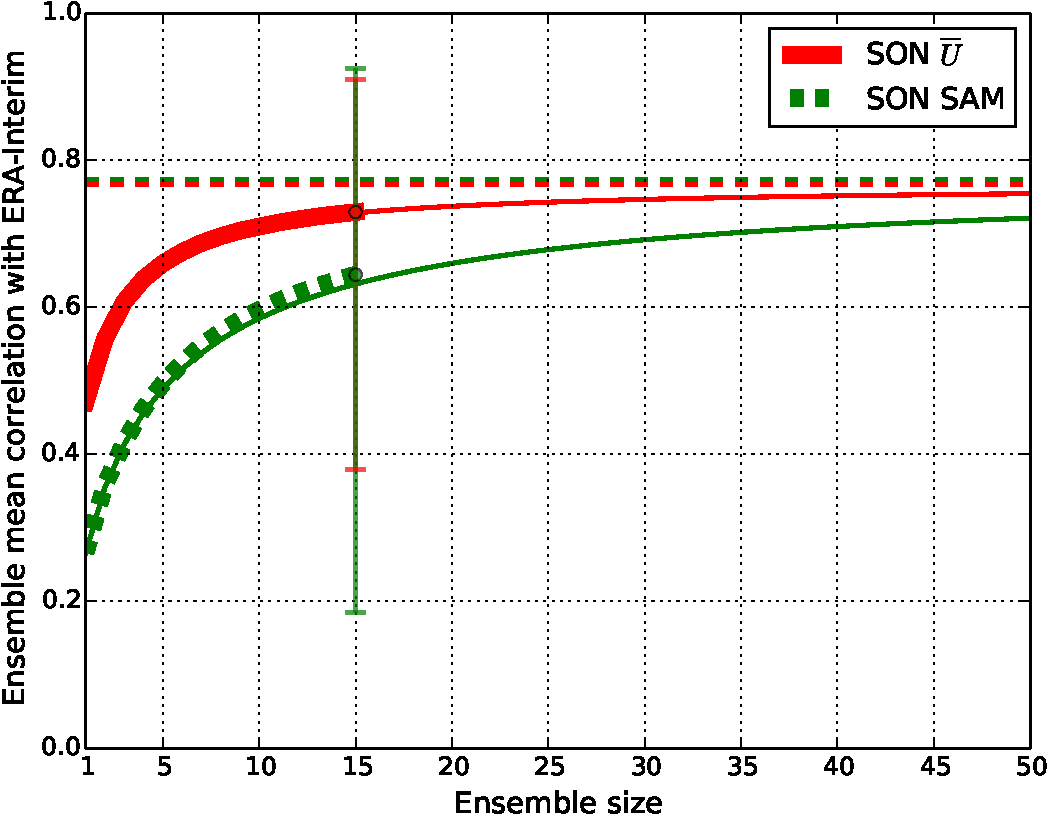
\includegraphics[width=0.6\textwidth,angle=0]{figures/chapter-seasonal/corr_ens_size_crop.pdf}\\
  \caption[Variation of GloSea5 forecast skill with ensemble size]{GloSea5
    ensemble mean correlation with ERA-Interim as a function of ensemble size
    for the SON mean $\overline{u}$ at 10~hPa and 60$^{\circ}$S and SON mean SAM
    (thick lines). A theoretical estimate of the variation of correlation with
    ensemble size is shown in each case (thin solid lines), along with its
    asymptote for an infinite sized ensemble (dashed lines). Error bars
    represent the 95\% uncertainty range for the correlation of the full
    15-member ensemble, calculated using a bootstrap
    test.}\label{fig:corr_ens_size_sh}
\end{figure}

Given the above result, it might be expected that more skilful predictions could
be obtained with a larger ensemble size. To illustrate the variation of hindcast
skill with ensemble size we systematically sample smaller sets of forecasts from
the full 15 members for each year, following the method of
\citet{Scaife2013}. This is repeated many times ($\sim 10~000$) and an average
value for a given sample size calculated. This variation of correlation skill
with ensemble size for both the SON mean SAM and stratospheric polar vortex
winds is shown in Figure \ref{fig:corr_ens_size_sh}. These curves closely follow
the theoretical relationship of \citet{Murphy1990}, which relies only on the
mean correlation between pairs of ensemble members, $\langle r_{\mathrm{mm}} \rangle$,
and the mean correlation between individual ensemble members and observations,
$\langle r_{\mathrm{mo}} \rangle$, given by
\begin{equation}
  r = \frac{\langle r_{\mathrm{mo}} \rangle \sqrt{n}}{\sqrt{1+(n-1)\langle r_{\mathrm{mm}} \rangle}}
  \, .
\end{equation} 
These curves are shown in Figure \ref{fig:corr_ens_size_sh}, along with their
asymptote for an infinite sized ensemble. This shows that the stratospheric
forecasts cannot be greatly improved with a larger ensemble size in the current
system, but greater correlation scores of the SAM could be achieved with an
ensemble size near 30. Although the large uncertainty range does not allow a
strong statement about potential predictability, the asymptote near 0.8 is
similar to that found by \citet{Scaife2013} using a longer hindcast and greater
ensemble size for the DJF NAO.

\subsubsection{Application to other seasons}

The dynamics of other seasons are different to those of the austral spring, so
results presented here for SON do not imply significant skill in prediction of
the SAM at other times. Indeed, the 1-month lead time ensemble mean correlation
of the DJF SAM with ERA-Interim is lower than that for SON at $r=0.39$ (95\%
confidence interval: [0.15,0.63]), as shown in Figure \ref{fig:djf_sam_ts}. The
low signal-to-noise ratio found in Figure \ref{fig:sam_ts} for SON can also be
seen in Figure \ref{fig:djf_sam_ts}. 

\begin{figure}[t]
  \noindent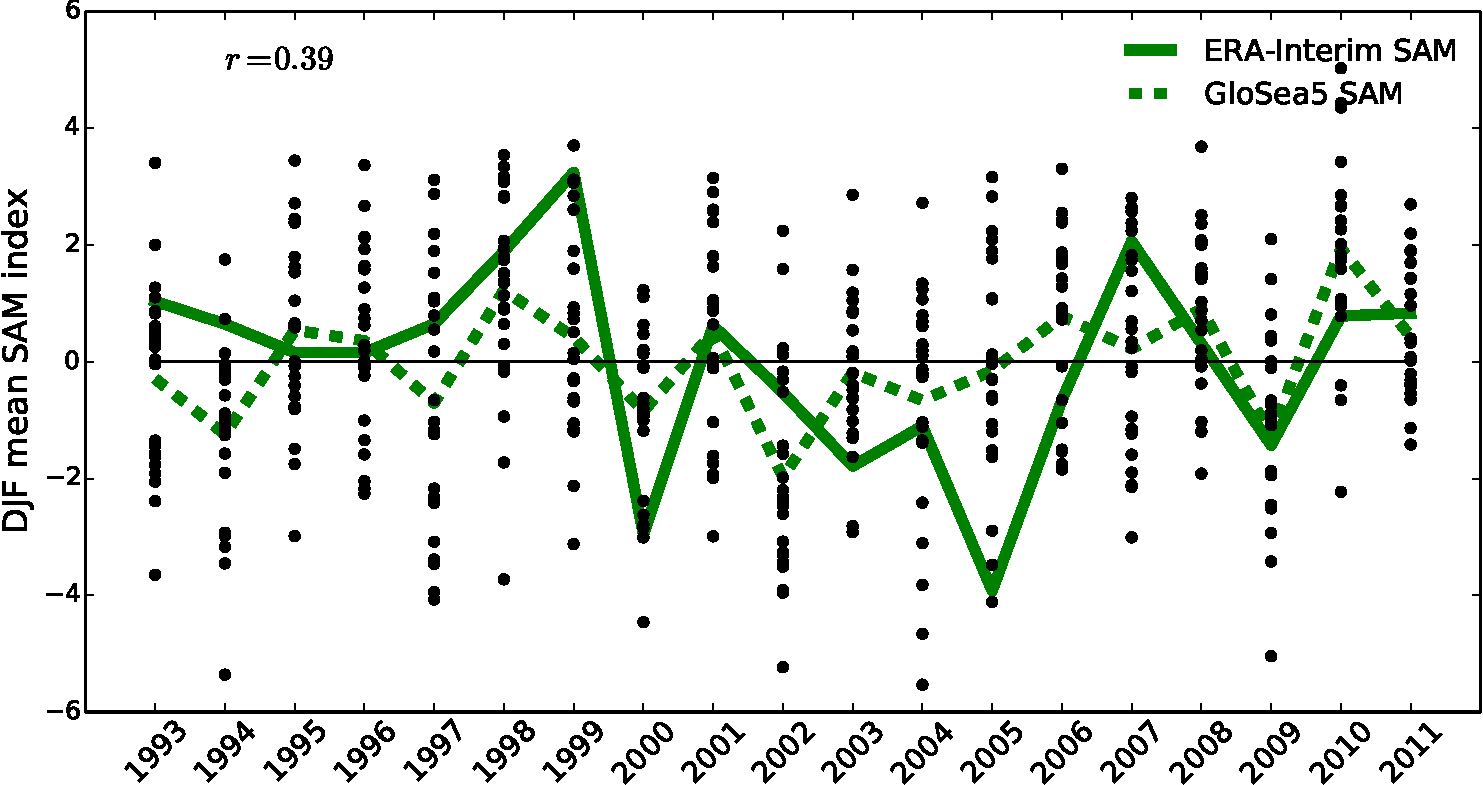
\includegraphics[width=\textwidth,angle=0]{figures/chapter-seasonal/DJF_SAM.pdf}\\
  \caption[GloSea5 predictions of the SAM.]{DJF mean Southern Annular Mode (SAM)
    index in individual GloSea5 hindcast ensemble members (dots), ensemble mean
    (dashed green curve) and ERA-Interim (solid green curve). The SAM is
    calculated from mean sea-level pressure data, and hindcasts initialised near
    1st November. The correlation of the ensemble mean and ERA-Interim values is
    0.39.}\label{fig:djf_sam_ts}
\end{figure}

\citet{Shaw2010} found that the strongest downward wave coupling between the
stratosphere and troposphere is present during September to December in the
SH. They attribute this to the fact that the lower stratospheric vortex is
westerly during this time, but the mid-upper stratospheric vortex is easterly
(because the final warming occurs first in the upper stratosphere) and acts as a
relecting surface for planetary waves. Following the final warming in the lower
stratosphere, \citet{Shaw2010} find wave coupling to be much
weaker. \citet{Shaw2011} extended this analysis to also demonstrate that the
dynamical influence of stratospheric ozone depletion on the troposphere through
wave coupling is greatest during September-December.

On the other hand, separate studies have found that the largest tropospheric
signals associated with stratospheric ozone depletion occur later, in DJF
\citep{WMO2010}. This may seem to contradict the findings of \citet{Shaw2010},
but the two results can be reconciled if a different mechanism is dominant at
this later time. Indeed, as well as an effect on the dynamical coupling between
the stratosphere and troposphere, \citet{Grise2009} proposed that stratospheric
ozone depletion can perturb radiative heating rates in the troposphere which
can, in turn, trigger changes in tropospheric dynamics. They used a radiative
model to investigate this effect and, importantly, found the largest influence
on polar tropospheric temperatures to occur during DJF. A possible physical
explanation for this is that it is only after the final warming, when the ozone
depleted polar stratospheric air is mixed with lower latitudes, that the
radiative effect on the troposphere is significant. While this was only an
idealised study which lacked tropospheric dynamics, it may suggest a
reconciliation with dynamical coupling being strongest from September-December
and radiative from December-February.

\begin{figure}[p] \vspace*{-3cm} \centering
   \noindent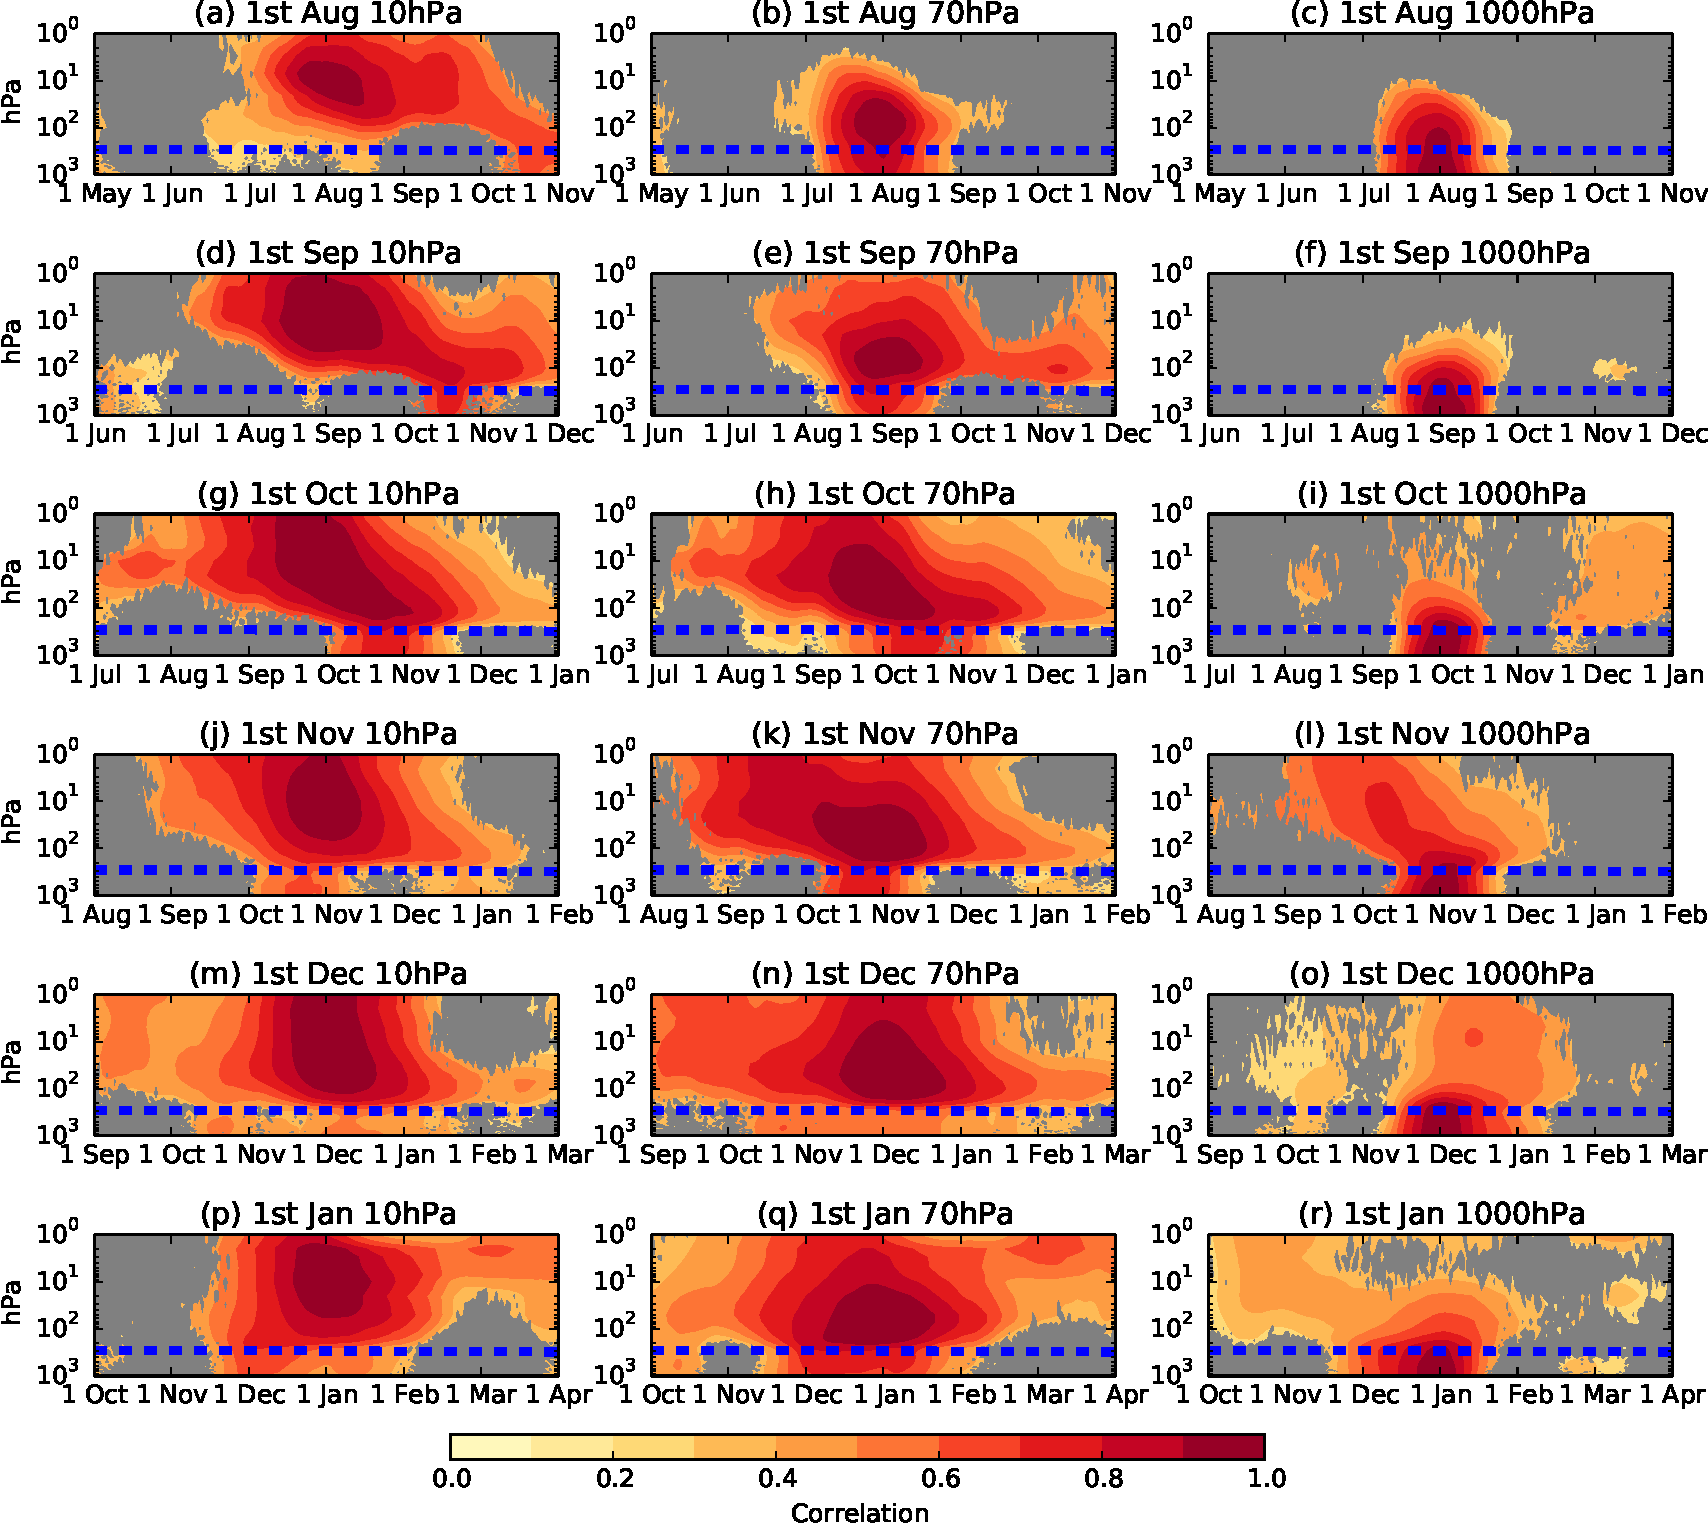
\includegraphics[width=\textwidth]{figures/chapter-seasonal/lag_height_corr_obs.pdf}
 \caption[Lag-height correlation of $Z'$ at 10~hPa and 1000~hPa.]{Correlation of
   ERA-Interim (1979--2010) Z' at 10~hPa, 70~hPa, and 1000~hPa with Z' at other
   times and lags. Values are smoothed with a 30-day running mean before
   correlations are calculated, and colours represent correlations that are 95\%
   significant from zero according to a bootstrap test.}
 \label{fig:lag_height_corr_obs}
\end{figure}

The time depedency of SH stratosphere-troposphere coupling is further
investigated in Figure \ref{fig:lag_height_corr_obs}. This shows lag-height
correlations of polar cap $Z'$ in the midstratosphere (10~hPa),
lower-stratosphere (70~hPa) and surface (1000~hPa) at the first of each month
from August--January using ERA-Interim data (1979--2010). As in Figure
\ref{fig:gph_lag_corr}, values are smoothed with a 30-day running mean before
correlations are calculated. Midstratosphere-leading significant correlations
with the October-November troposphere are seen from 1st August (Figure
\ref{fig:lag_height_corr_obs}(a)), as also shown in Figure
\ref{fig:gph_lag_corr}. Furthermore the strongest negative lag correlations of
the surface with the stratosphere occur at 1st November (Figure
\ref{fig:lag_height_corr_obs}(l)). This supports the result of
\citet{Shaw2010} that September-December is the time of strongest
stratosphere-troposphere dynamical coupling. 

Similar, but weaker lag correlations are seen at 1st Janurary (Figure
\ref{fig:lag_height_corr_obs}(r)). This is unlikely to be due to dynamical
coupling since it comes after the stratospheric final warming, and so may be a
result of the radiative effect described above. It is important to note that
GloSea5 does not contain interactive ozone chemistry, so the radiative effects
of ozone variability will not be captured by the model. This may explain, to
some extent, the reduced skill in the prediction of DJF SAM compared to the SON
SAM, since the predictable effects of the stratosphere on the troposphere are
not captured during DJF. Consequently, more skilful forecasts of the DJF SAM may
be possible with a model including interactive ozone chemistry. 



\section{Conclusions}
\label{sec:seas-conclusions}

Motivated by the results of Chapters \ref{cha:moments} and \ref{cha:models}, we
have analysed the predictability of the polar stratosphere and its influence on
the troposphere in a set of hindcasts produced by a stratosphere-resolving
seasonal prediction system. Analsysis has focussed on the NH for the boreal
winter (DJF) and SH for the austral spring (SON), with forcasts initialised at a
1-month lead time.

No statistically significant skill was found in the prediction of the seasonal
mean strength of the NH stratospheric polar vortex, or the occurrence of SSWs,
split or displaced vortex events. This result may be surprising given that the
same system produces skilful hindcasts of the winter NAO, which is known to
influence the polar stratosphere. It does, however, suggest that this NAO skill
is unlikely to be influenced by the stratosphere and may be attributable to
other model improvements.

On the other hand, skillful prediction of the interannual variability of the
spring Antarctic stratospheric polar vortex at seasonal lead times. This
includes capturing an increased likelihood of the 2002 SSW which is the most
extreme year in the ensemble mean and has the only ensemble member in 14 years
which simulates a SSW (although another is close to simulating a SSW in
1997). Because this variability is observed to be closely correlated with
Antarctic column ozone amounts, we are able to perform skillful predictions of
interannual variability in Antarctic ozone depletion.

We also find significant skill in hindcasts of the spring mean SAM index.  By
studying the variation of this skill with time and height, we suggest that this
skill is influenced by stratospheric anomalies which descend with time and are
coupled with the troposphere in October and November. In fact, the influence of
the stratosphere is such that skillful statistical predictions of the October
SAM can be made using only information from 1st August in the mid-stratosphere.

Assuming that the 14 year period studied here is representative of future years,
these results suggest that it may now be possible to make skillful seasonal
forecasts of interannual variations in springtime ozone depletion and large
scale weather patterns across the Southern Hemisphere.




\pagebreak

\begin{subappendices}
\section{Choice of time period for statistical forecast}
\label{sec:app-choice-time-period}

The aim of the LOOCV statistical analysis presented in Section
\ref{sec:seas-strat-trop-coupl} was to estimate the degree of predictability
which arises from both the midstratosphere at the start of August and the
July-mean Ni\~no-4 index. Importantly, this analysis used the longer ERA-Interim
period of 1979-2009 rather than the same 1996-2010 period over which the
hindcast simulations were run. A choice of the longer period would be
justafiable (and, indeed, preferable) if the relationships between these
parameters and the forecast perameter ($Z'$) are not physically different over
the shorter period. That is, if the shorter period is a marginal distribution of
the longer period. This is shown to be the case below.

We use the monthly Southern Oscillation Index (MSLP difference between Darwin
and Tahiti, which is highly correlated with the Ni\~no-4 index) data obtained
from the Australian Bureau of Meteorology
(\url{http://www.bom.gov.au/climate/current/soihtm1.shtml}), and a station-based
SAM index from the British Antarctic Survey \citep{Marshall2003}. For the
1996-2009 hindcast period we find the correlation of June-July SOI with Oct-Nov
SAM to be $r=0.63$. For 1979-2010 (the ERA-Interim period) $r=0.32$. In order to
justify using the shorter hindcast period (with higher correlation), it would
need to be the case that the SAM/SOI correlation is statistically significantly
stronger during the hindcast period than the ERA-Interim period, so that these
different correlations are not a result of random variability.

To test whether this is the case, we use a bootstrap test which randomly samples
(with replacement) 14 years of detrended SAM and SOI from 1979-2013, and
calculates the correlation. Figure \ref{fig:sam_soi_corr} shows a histogram of
these correlations along with the 1996-2009 correlation. The 1996-2009 value is
not inconsistent with random variability at the 95\% level for either a one- or
two-tailed test. Therefore we conclude that the SAM/SOI correlation is not
statistically significantly greater for 1996-2009. As such the 1996-2009
correlation is a marginal distribution of 1979-2013 so we include the longer
ERA-Interim period in our analysis to provide a more robust measure of sources
of predictability. 

For completeness we include a figure with the same analysis limited to
1996--2009 in this appendix (Figure \ref{fig:lag_height_short}). Similar
features as Figure \ref{fig:gph_lag_corr} can be seen although tropospheric
skill emerges later in Figure \ref{fig:lag_height_short}(b) and earlier in
Figure \ref{fig:lag_height_short}(c).

% (and for the full 1957-2013 extent of the SAM record, $r=0.01$)

\begin{figure}[t]
  \centering
  \noindent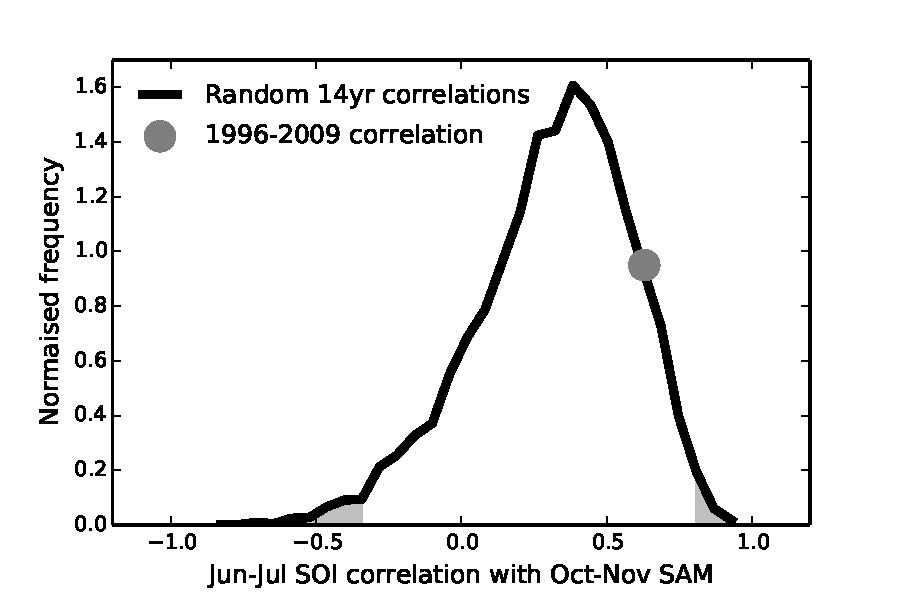
\includegraphics[width=0.7\textwidth,angle=0]{figures/chapter-seasonal/SAM_SOI_corr.pdf}\\
  \caption[Correlation of the SOI with the SAM.]{Histogram of correlations of
    random 14-year samples of detrended June-July SOI with October-November
    SAM. Also shown is the correlation over the 1996--2009 hindcast period. Grey
  shading indicates the $<2.5$\% and $>97.5$\% ranges.}\label{fig:sam_soi_corr}
\end{figure}

\begin{figure}[t]
  \noindent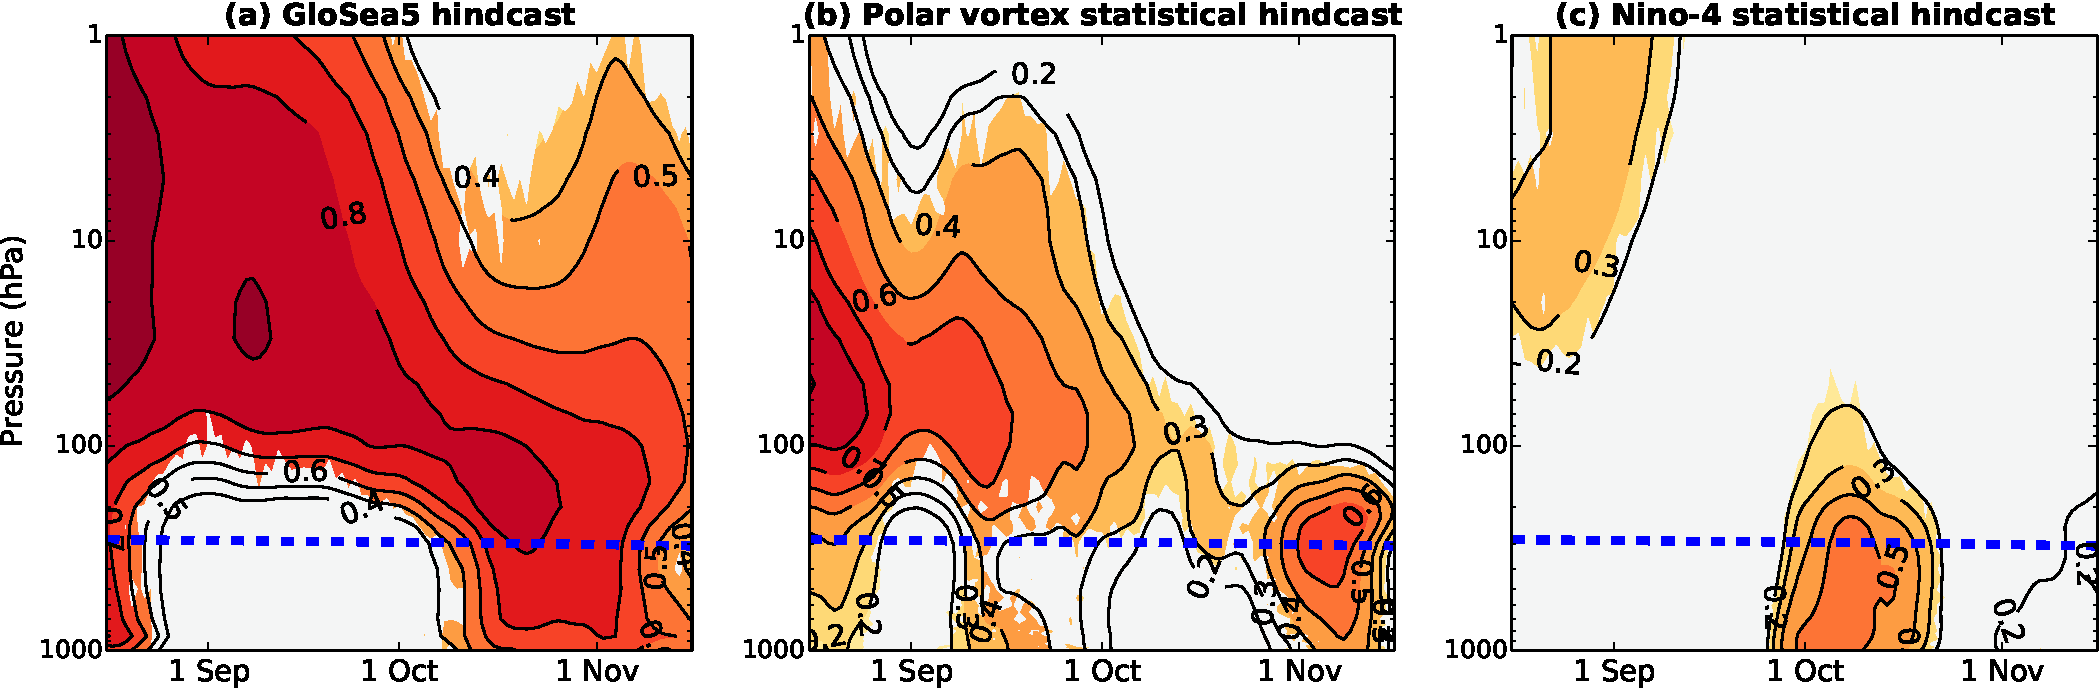
\includegraphics[width=\textwidth,angle=0]{figures/chapter-seasonal/lag_height_short.pdf}\\
  \caption[Lag-height correlation of GloSea5 polar cap geopotential height]{As
    Figure \ref{fig:gph_lag_corr} but all analysis restricted to the 1996--2009
    period.}\label{fig:lag_height_short}
\end{figure}

\end{subappendices}


%%% Local Variables:
%%% mode: latex
%%% TeX-master: "thesis"
%%% End:
